\styledchapter{Ordinary Least Squares Estimation}

\section{Best Predictors and Linear Approximation}

\begin{theorem}	Suppose $\E\left[y^2\right]<\infty$ and $\E\left[x_j^2\right]<\infty$ for each $j=1,\ldots,k$. The function $g(x):=\E\left[y\mid x\right]$ is the best predictor of $y$ given $x$ under square loss. That is:
	\[
		\E\left[y\mid x\right]\in\argmin_g \E\left[(y-g(x))^2\right].
	\]
\end{theorem}

\begin{remark}	We can interpret the linear model as a best linear approximation to the conditional expectation, if we don't believe the conditional expectation is linear:
	\[
		\E\left[y\mid x\right]\approx x'\beta.
	\]
	We choose $\beta$ to solve
	\[
		\min_{b\in\R^k}\E\left[\left(\E\left[y\mid x\right]-x'b\right)^2\right].
	\]
	The solution is the best linear approximation to $\E\left[y\mid x\right]$ under square loss.
\end{remark}

\begin{figure}[htpb]
	\centering
	\caption{Sample average at each $x$ ($\approx \E\left[Y \mid X\right]$, the conditional mean) and best linear approximation to conditional mean}
	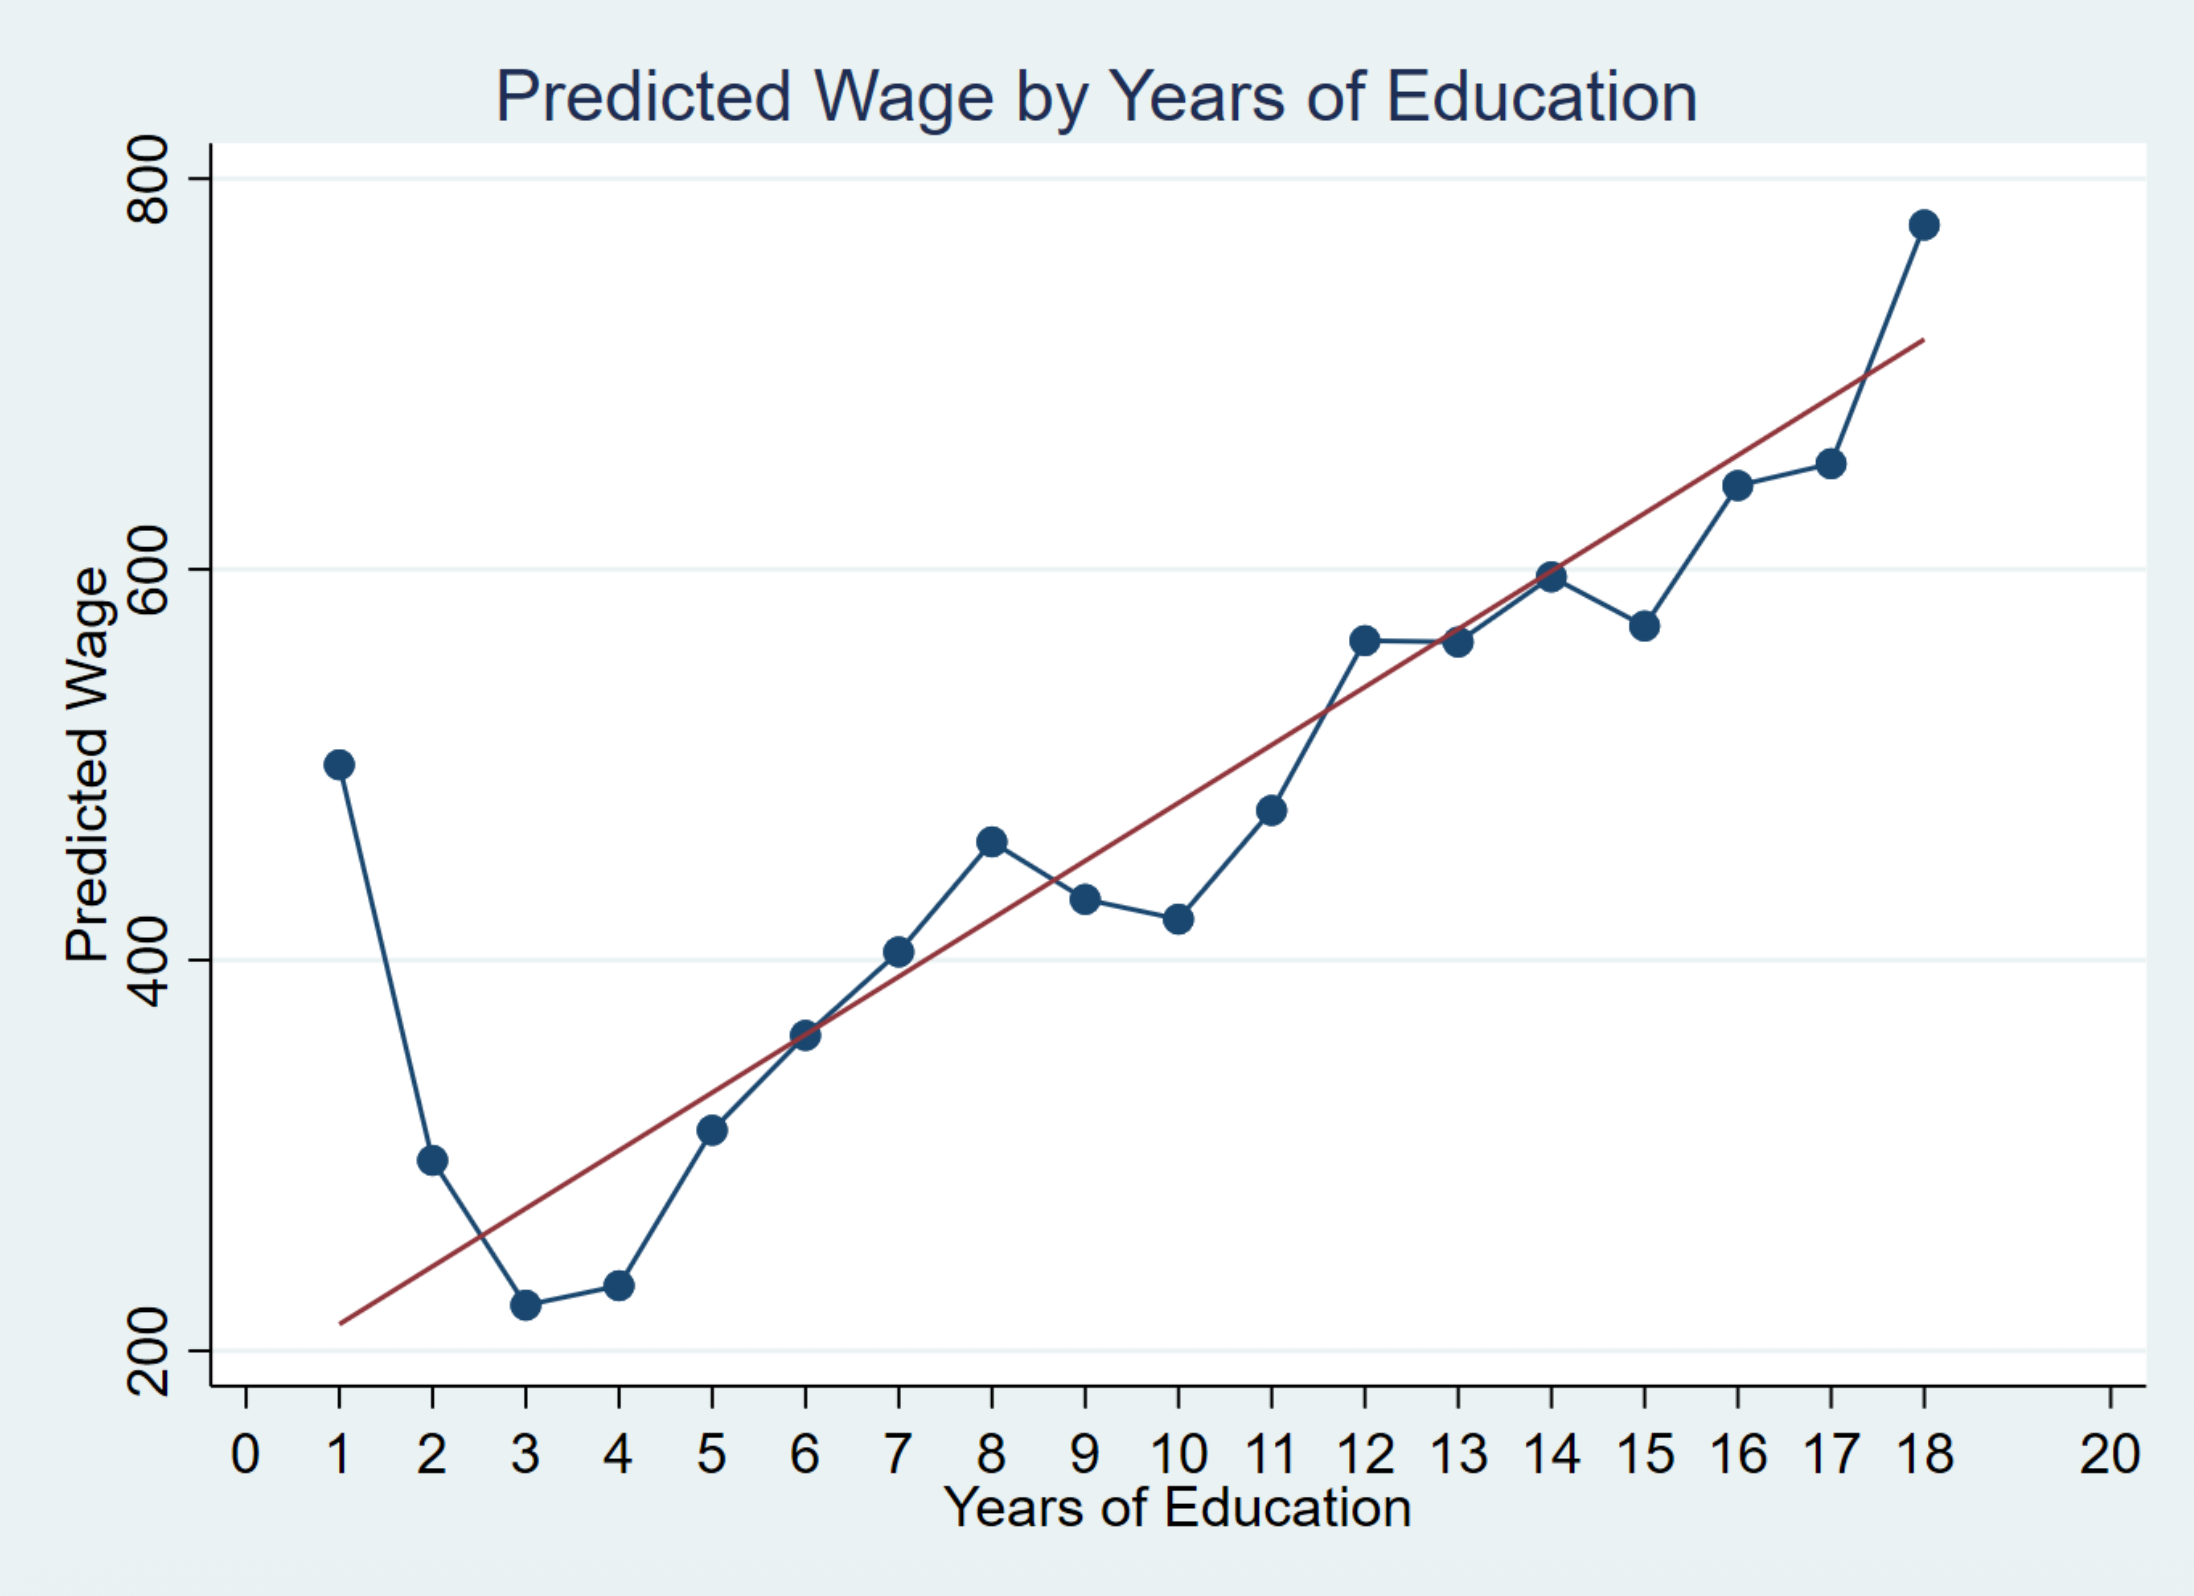
\includegraphics[width=0.78\textwidth]{images/1-22-1}
\end{figure}

There is a small sample problem for years of education less than 8. We trade off variance at this low end, getting a higher bias.

\begin{definition}[Best Linear Predictor]
	The best linear predictor of $y$ given $x$ is defined by
	\[
		\beta=\E\left[xx'\right]^{-1}\E\left[xy\right],
	\]
	where the FOC implies $\E\left[xy\right]=\E\left[xx'\right]\beta$. In order for these equations to have a unique solution, $\E\left[xx'\right]$ must be full rank/invertible. This is equivalent to there being no perfect multicollinearity in $x$; i.e., there is no $a\in \R^k\setminus \{0\}$ such that $x'a = 0$ with probability $1$.
\end{definition}

\section{OLS Estimation}

\begin{remark}	Given a sample $\{y_i,x_i\}_{i=1}^n$, we can apply the sample analogue principle\footnote{Now, $\theta(f)$ is defined as an $\argmin$ of an objective function. We find $\theta(\hat{f})$ now.} and solve the analogous in-sample problem:
	\[
		\min_{b\in\R^k}\frac{1}{n}\sum_{i=1}^n\left(y_i-x_i'b\right)^2
	\]
	to yield an estimator of $\beta$.\boxednote{The solution is $\hat{\beta} = (\frac{1}{n} \sum_i X_iX_i')^{-1} \frac{1}{n} \sum_i X_i Y_i$.} The first order conditions with respect to each $b_j$ imply that at the solution\boxednote{We think of a matrix of $x$ with the rows as observations $1:n$ and the columns as dimensions of $x$ from $1:k$. The first column will be $\vec 1$. Basically, we attach a $1$ to the meaningful characteristics of $x_i$ to get the intercept $\beta_0$ when multiplying by $X$. For example, if we want to consider predicting house price with number of bedrooms, a house would be represented by $(x_i;ly_i) = (1, \text{rooms}; \text{price})$. We want to allow the prediction line to not pass through the origin so the $\beta$s are interpretable as partial covariances.}:
	\[
		-2\cdot\frac{1}{n}\sum_{i=1}^n x_{ij}\left(y_i-x_i'\hat\beta\right)=0\quad\text{for all }1\le j\le k.
	\]

	Stacking these first order conditions gives
	\[
		\begin{pmatrix}
			\frac{1}{n}\sum_{i=1}^n x_{i1}(y_i-x_i'\hat\beta) \\
			\vdots                                            \\
			\frac{1}{n}\sum_{i=1}^n x_{ik}(y_i-x_i'\hat\beta)
		\end{pmatrix}
		=
		\frac{1}{n}\sum_{i=1}^n x_i(y_i-x_i'\hat\beta)=0.
	\]

	Adding $\left( \frac{1}{n} \sum_i x_i x_i' \right)\hat{\beta}$, we get that the FOCs imply
	\[
		\frac{1}{n}\sum_{i=1}^n x_iy_i=\left(\frac{1}{n}\sum_{i=1}^n x_ix_i'\right)\hat\beta.
	\]
	Provided $\frac{1}{n}\sum_{i=1}^n x_ix_i'$ is invertible, which occurs iff none of the columns $x_{\cdot j}$ are collinear, we obtain\boxednote{We can think of $(X_i,Y_i) \in \R^{k+1}$ so our estimator is an object in $\R^{k}$.}
	\[
		\hat\beta=\left(\frac{1}{n}\sum_{i=1}^n x_ix_i'\right)^{-1}\frac{1}{n}\sum_{i=1}^n x_iy_i.
	\]
\end{remark}

\begin{definition}[Fitted Values and Residuals]
	The $i$-th fitted value is:
	\[
		\hat y_i=x_i'\hat\beta.
	\]
	The $i$-th residual is
	\[
		\hat u_i=y_i-\hat y_i.
	\]
\end{definition}

\begin{remark}[FOC of OLS]
	The first order condition of the least squares minimization problem implies
	\[
		\sum_{i=1}^n x_i(y_i-x_i'\hat\beta)=\sum_{i=1}^n x_i\hat u_i=0.
	\]
	We can write this compactly as $X'\hat{u} = 0$.
\end{remark}

\begin{example}[Simple Linear Regression]
	Consider the simple linear model:
	\[
		y=\beta_0+\beta_1x_1+u,
	\]
	where now $x=(1,x_1)'$, and $\beta=(\beta_0,\beta_1)'$. Our earlier work implies\boxednote{Note that this expression for $\beta$ holds regardless of the dimension of $X$.}
	\[
		\beta=\E\left[xx'\right]^{-1}\E\left[xy\right].
	\]
	We have
	\begin{align*}
		\E\left[xx'\right]^{-1}
		&=\begin{pmatrix}
			1   & x_1   \\
			x_1 & x_1^2
		\end{pmatrix}^{-1}
		=\frac{1}{\E\left[x_1^2\right]-\E\left[x_1\right]^2}\begin{pmatrix}
			\E\left[x_1^2\right] & -x_1 \\
			-x_1                 & 1
		\end{pmatrix}, \\
		\E\left[xy\right]
		&=\begin{pmatrix}
			\E\left[y\right] \\
			\E\left[x_1y\right]
		\end{pmatrix}.
	\end{align*}
	It follows that\boxednote{\texthl{apparently this was done in the hw??}}
	\[
		\beta=\frac{1}{\operatorname{Var}(x_1)}\cdot\begin{pmatrix}
			\E\left[x_1^2\right] & -\E\left[x_1\right] \\
			-\E\left[x_1\right]  & 1
		\end{pmatrix}\begin{pmatrix}
			\E\left[y\right] \\
			\E\left[x_1y\right]
		\end{pmatrix}
		=\begin{pmatrix}
			\E\left[y\right]-\beta_1\E\left[x_1\right] \\
			\frac{\operatorname{Cov}(y,x_1)}{\operatorname{Var}(x_1)}
		\end{pmatrix}.
	\]
\end{example}

\begin{remark}[Slope Parameter and Correlation]
	Notice that
	\[
		\beta_1=\frac{\operatorname{Cov}(W,S)}{\operatorname{Var}(S)}=\sqrt{\frac{\operatorname{Var}(W)}{\operatorname{Var}(S)}}\cdot\operatorname{Corr}(W,S),
	\]
	so the slope coefficient is proportional to the correlation between wages and education (likely $>0$).

	Notice that increasing $\operatorname{Var}(W)$ stretches the scatter plot vertically (but leaves the correlation unchanged). The slope coefficient should increase in magnitude.

	Increasing $\operatorname{Var}(S)$ stretches the scatter plot horizontally (but leaves the correlation unchanged). The slope coefficient should decrease in magnitude.
\end{remark}

\begin{example}[Changing units of measurement]
	Suppose wages are now measured in cents per hour rather than dollars per hour. Let $\tilde W$ denote wages in cents:
	\[
		\tilde W=100W.
	\]
	Find the best linear predictor of $\tilde W$ given $S$, i.e. find $(\alpha_0,\alpha_1)$ such that\boxednote{\texthl{ why is including the condition on the expectation of $SU$, $U$ and finding the best linear predictor equivalent to the minimization problem without the error term?}}
	\[
		\tilde W=\alpha_0+\alpha_1S+U;\qquad \E\left[SU\right]=\E\left[U\right]=0.
	\]
	Find that
	\[
		\alpha_1=\frac{\operatorname{Cov}(\tilde W,S)}{\operatorname{Var}(S)}=\frac{100\operatorname{Cov}(W,S)}{\operatorname{Var}(S)}=100\beta_1,
	\]
	\[
		\alpha_0=\E\left[\tilde W\right]-\alpha_1\E\left[S\right]=100(\E\left[W\right]-\beta_1\E\left[S\right])=100\beta_0.
	\]
\end{example}

\begin{example}[Simple Linear Regression Estimation]
	Write the model for each individual $i=1,\ldots,n$ in the sample:
	\[
		y_i=\beta_0+\beta_1x_{i1}+u_i,
	\]
	and estimate the parameters using ordinary least squares:
	\[
		\hat\beta=\left(\frac{1}{n}\sum_{i=1}^n x_ix_i'\right)^{-1}\frac{1}{n}\sum_{i=1}^n x_iy_i
		=\begin{pmatrix}
			\bar y_n-\hat\beta_1\bar x_{1,n} \\
			\frac{\frac{1}{n}\sum_{i=1}^n x_{i1}y_i-\bar x_{1,n}\cdot\bar y_n}{\frac{1}{n}\sum_{i=1}^n x_{i1}^2-(\bar x_{1,n})^2}
		\end{pmatrix}.
	\]
\end{example}

\section{Matrix Notation and Projection}

\begin{remark}[Matrix Notation]
	First write the model for each observation $i=1,\ldots,n$:
	\[
		y_i=x_i'\beta+u_i.
	\]
	Stack the observations into matrices:
	\[
		\begin{pmatrix}
			y_1    \\
			y_2    \\
			\vdots \\
			y_n
		\end{pmatrix}
		=
		\underbrace{\begin{pmatrix}
			-x_1'- \\
			-x_2'- \\
			\vdots \\
			-x_n'-
		\end{pmatrix}}_{\text{design matrix}}
		\beta
		+
		\begin{pmatrix}
			u_1    \\
			u_2    \\
			\vdots \\
			u_n
		\end{pmatrix}.
	\]
	Therefore
	\[
		Y=X\beta+U,
	\]
	where the matrix $X$ is called the design matrix, with columns $X_1,\ldots,X_k\in\R^n$. If we have an intercept, then the first feature $X_1$ is a column of $1$s.

	The least squares minimization problem is
	\[
		\min_{b\in\R^k}\sum_{i=1}^n(y_i-x_i'b)^2\equiv\min_{b\in\R^k}(Y-Xb)'(Y-Xb) = \min_{B \in \R^k} \|Y - Xb\|^2
	\]
	because the sum of squares is just the inner product of $Y-Xb$ with itself.
	To see this, write \[
		\R^n \ni Y - Xb = \begin{bmatrix}
		y_1-x_1'b \\
		\vdots \\
		y_n - x_n'b
		\end{bmatrix} 
	,\] so \[
	\left( Y-Xb \right)'(Y-Xb) = \sum\limits_{i=1}^{n} \left( y_i - x_i'b \right)^2
	.\] Hence, we want to pick $b$ to minimize the distance from $Xb \in \operatorname{Span}(X)$ to $Y\in \R^n$ in the Euclidean norm. This is the point that is the orthogonal projection of $Y$ onto $\operatorname{Span}(X)$.

	We can expand the objective function as
	\[
		(Y-Xb)'(Y-Xb)=Y'Y-Y'Xb-b'X'Y+b'X'Xb=Y'Y-2Y'Xb+b'X'Xb,
	\]
	so the first order condition with respect to $b_j$ is
	\[
		-2\sum_{i=1}^n y_i\cdot x_{ij}+2\sum_{i=1}^n x_{ij}\cdot x_i'\hat\beta=0.
	\]
	Stack the first order conditions into a $k\times 1$ vector:
	\[
		-2\sum_{i=1}^n y_i\cdot x_i+2\left[\sum_{i=1}^n x_ix_i'\right]\hat\beta=0;\quad\text{or}\quad
		-2X'Y+2X'X\hat\beta=0.
	\]
	This yields $X'\left( Y- X\hat{\beta} \right) = 0$,\footnote{This says that every column of $X$ (row of $X'$) is orthogonal to the residual (row).} which is equivalent to (provided $X$ is full column rank):
	\[
		\hat\beta=(X'X)^{-1}X'Y.
	\]
\end{remark}

\begin{remark}	We have used the fact that
	\[
		\sum_{i=1}^n x_ix_i'=X'X,\qquad
		\sum_{i=1}^n y_ix_i=X'Y.
	\]
	To see why these identities hold, consider $X \in \R^{n\times k}$ and $X' \in \R^{k\times n}$, so \[
		X'X = \begin{bmatrix}
			\sum\limits_{i=1}^{n} x_{i_1}^2 & \sum\limits_{i=1}^{n} x_{i 1} x_{i 2} & \cdots \\
		\sum\limits_{i=1}^{n} x_{i 2}x_{i 1} & \sum\limits_{i=1}^{n} x_{i 2}^2 & \cdots \\
		\vdots & & \ddots
		\end{bmatrix} = \sum\limits_{i=1}^{n} X_i X_i'
	.\] Switching a transpose between matrices and vectors moves the transpose.

	The vector of fitted values is $\hat Y=X\hat\beta$, and the vector of residuals is $\hat U=Y-\hat Y$. The FOC of the least squares problem is equivalently written as $X'\hat U=0$. These are the normal equations.
\end{remark}

\begin{proposition}	$(X'X)^{-1}$ exists iff $X$ is full column rank.

	If $X$ is not full column rank, there exists $c\neq 0$ such that $Xc=0$, so $X'Xc=0$, implying $X'X$ is not invertible.

	If $X'X$ is not invertible, there exists $a\neq 0$ such that $X'Xa=0$, so $a'X'Xa=0$. But
	\[
		a'X'Xa=[Xa]'(Xa),
	\]
	which is a sum of squares which equals zero iff $Xa=0$. Since $a\neq 0$, $X$ is not full rank.

	In a simple linear regression, need there to be some variation in $\left( X_i \right)_{1:n}$ so it isn't collinear with the constant. Equivalently, need $\det(X'X)=(n-1)\cdot\widehat{\operatorname{Var}}(x)\neq 0$. When $X_i \in R^2$ with a column of $1$s, then we require that the 2nd column of $X$ is not identically some constant.
\end{proposition}

\begin{theorem}[Projection Theorem]
	Let $y\in\R^n$ and let $S$ be any nonempty subspace of $\R^n$ equipped with the dot product. There exists a unique point $\hat y$ such that $\|y-\hat y\|$ is minimized over $S$.\boxednote{Here, we are thinking of $S$ as a $k$-dimensional subspace of $\R^n$ --- the subset of $\R^n$ spanned by the columns of $X$.} A necessary and sufficient condition for $\hat y$ is that $\hat{y} \in S$ and $\hat y-y$ is orthogonal to every vector in $S$.

	By definition of $\hat\beta$, the vector $X\hat\beta$ is the closest (in the Euclidean norm) to $Y$ in the set of all vectors
	\[
		\{Xb:b\in\R^k\}=S(X),
	\]
	where $S(X)$ denotes the span of the columns of $X$. Given a vector $Y\in\R^n$ and a matrix $X\in\R^{n\times k}$, the projection of $Y$ onto $S(X)$ is the vector\footnote{We previously found $v^* = X\hat{\beta}$.}
	\[
		v^*\in\argmin_{v\in S(X)}\|Y-v\|^2.	
	\]

	While the coefficients $\hat{\beta}$ may not be unique (if $X$ is not full column rank), this theorem guarantees that $X\hat{\beta}$ is unique. 
\end{theorem}

\begin{example}	We can draw the following to provide intuition. Consider $n=2$, $k=2$, and a model with no intercept, so $y_i = \beta x_i + u_i$. Suppose $X = \begin{pmatrix}
	x_1 \\
	x_2
	\end{pmatrix} = \begin{pmatrix}
	1 \\
	0
	\end{pmatrix} $ and $Y = \begin{pmatrix}
	3 \\
	3
	\end{pmatrix} $.

	In this case, $S(X) = \{c \begin{pmatrix}
	1 \\
	0
	\end{pmatrix} : c\in \R\}$, so \[\hat{Y} = P_X Y = \begin{pmatrix}
	3 \\
	0
	\end{pmatrix}, \quad\hat{U} = \begin{pmatrix}
	0 \\
	3
\end{pmatrix}.\]

	We note that $P_X Y$ is the closest point to $Y$ in $S(X)$, while $\hat{U}$ is orthogonal to $S(X)$.
\end{example}


\begin{remark}	Restricting the minimizer to vectors in $S(X)$, the necessary and sufficient condition for the minimizer is
	\[
		x'(Y-\hat Y)=0
	\]
	for all $x\in S(X)$. Since the columns of $X$ are a basis of $S(X)$, this condition is equivalent to
	\[
		X'(Y-\hat Y)=0.
	\]
	$\hat Y\in S(X)$ means $\hat Y=Xb$ for some $b\in\R^k$. Thus
	\[
		X'Y=X'Xb\implies b=(X'X)^{-1}X'Y\implies\hat Y=X(X'X)^{-1}X'Y.
	\]
	That is, the projection of $Y$ onto $S(X)$ is given by $\hat Y=P_XY$, where $P_X$ is the projection matrix defined below.
\end{remark}

\begin{definition}[Projection Matrix]
	Since $X\hat\beta=X(X'X)^{-1}X'Y$, we call $P_X=X(X'X)^{-1}X'$ the projection matrix (it projects $Y$).

	The projection matrix is symmetric:
	\[
		P_X'=[X(X'X)^{-1}X']'=X[(X'X)^{-1}]'=X[(X'X)']^{-1}X'=P_X.
	\]
\end{definition}

\begin{remark}	$P_X$ is also idempotent (meaning $P_X\cdot P_X=P_X$), since:
	\[
		P_XP_X=X(X'X)^{-1}X'X(X'X)^{-1}X'=X(X'X)^{-1}X'=P_X,
	\]
	which reflects the fact that after a vector has been projected on to the span of the columns of $X$, it does not change as a result of the second projection. This is because the projected vector is already a linear combination of the columns of $X$.
\end{remark}

\begin{definition}[Residual Maker Matrix]
	The residual of the projection of $Y$ onto the columns of $X$ is
	\[
		Y-\hat Y=Y-P_XY=(I_n-X(X'X)^{-1}X')Y.
	\]
	Therefore, the matrix $M_X:=I_n-X(X'X)^{-1}X' = I_n - P_X$ is called the residual maker.

	$M_XY$ is the residual of the projection of $Y$ onto the space spanned by the columns of $X$.
\end{definition}

\begin{proposition}[Properties of Residual Maker]
	$M_X$ projects a vector onto the $n-k$ dimensional vector space orthogonal to the column space of $X$. This is called the orthogonal complement of $S(X)$.

	The residual of the projection $M_X y$ is $y - M_X y = P_X y \in S(X) \perp OC(S(X))$.

	Some properties:
	\begin{itemize}
		\item $P_XM_X=M_XP_X=0$, since $P_X(I-P_X)=P_X-P_XP_X=0$.
		\item $P_XX=X(X'X)^{-1}X'X=X$: Projecting $X$ onto its own span does nothing.
		\item $M_XX=X-P_XX=0$: Residual of projecting $X$ onto its own span is $0$.
		\item For any vector $y$, $y=P_Xy+M_Xy=\hat y+\hat u$.
	\end{itemize}
\end{proposition}

\section{$R^2$ and Goodness of Fit}

\begin{definition}[$R^2$]
	\begin{itemize}
		\item $\sum_{i=1}^n(y_i-\bar y)^2:=\text{TSS}$ is called the total sum of squares.
		\item $\sum_{i=1}^n(y_i-x_i'\hat\beta)^2:=\text{SSR}$ is the sum of squared residuals.
		\item $\sum_{i=1}^n(\hat y_i-\bar y)^2:=\text{ESS}$ is the explained sum of squares.
	\end{itemize}
	The coefficient of determination ($R^2$) is given by
	\[
		R^2=\frac{\text{ESS}}{\text{TSS}}.
	\]
\end{definition}

\begin{remark}	Immediately, we see that $SSR \le TSS$ because the $SSR$ is the residuals from letting our line of fit to have a free intercept and slope, while $TSS$ fixes a slope of $0$.
	$R^2$ measures how well OLS estimation of a linear model which includes a constant as a regressor fits a given dataset relative to a model only containing a constant. In other words, we are comparing two models:
	\begin{enumerate}[label=(\roman*)]
		\item $y = \beta_0 + u$, which implies $\hat{\beta}0^{OLS} = \overline{y}$
		\item $y = \beta_0 + \beta_1 x + \epsilon$,
	\end{enumerate}
	and seeing what fraction the SSR of the second model is of the SSR of the first model.
	

	We have:
	\[
		R^2=\frac{\text{ESS}}{\text{TSS}}=\frac{\sum_{i=1}^n(\hat y_i-\bar y_n)^2}{\sum_{i=1}^n(y_i-\bar y_n)^2}=1-\frac{\sum_{i=1}^n(y_i-x_i'\hat\beta)^2}{\sum_{i=1}^n(y_i-\bar y_n)^2},
	\]
	where the third equality follows from $SSR + ESS = TSS$ (shown later).

	The second and third equalities imply $0\le R^2\le 1$.

	$R^2=1$ iff $\text{SSR}=0$, which means $\hat U=0$.

	$R^2=0$ iff $\text{SSR}=\text{TSS}$, which implies all $y_i$ are identical and $\hat\beta=(\bar y,0,\ldots,0)$ provided $X$ is full column rank. In this case the model fits the data no better than a constant would; knowing $x$ does not help us predict $y$.
\end{remark}

\begin{proof} (Decomposition of $R^2$)
	Let $P_c=\mathbf{1}(\mathbf{1}'\mathbf{1})^{-1}\mathbf{1}'=\frac{1}{n}\mathbf{1}\mathbf{1}'$ be the projection matrix onto the span of the column vector of ones in $\R^n$. Then $P_cY=\frac{1}{n}\mathbf{1}\mathbf{1}'Y=\bar y_n\mathbf{1}$, so:
	\begin{align*}
		\text{TSS}&=\|Y-P_cY\|^2=\|M_cY\|^2 \\
		\text{ESS}&=\|P_XY-P_cY\|^2=\|P_XY-P_XP_cY\|^2=\|P_XM_cY\|^2 \\
		\text{SSR}&=\|Y-P_XY\|^2=\|M_XY\|^2=\|M_XM_cY\|^2.
	\end{align*}\boxednote{We see that \begin{align*}
		M_X M_c Y &= M_X Y - M_X P_c Y \\
		           &= M_X Y,
	\end{align*}since $P_c Y\in S(X)$ means $M_X P_c Y=0$.}

	Finally, since $P_XM_cY \in S(X)$ and $M_XM_cY \in OC(S(X))$ are orthogonal:
	\[
		\|M_XM_cY\|^2+\|P_XM_cY\|^2=\|M_XM_cY+P_XM_cY\|^2=\|M_cY\|^2,
	\]
	so $\text{ESS}+\text{SSR}=\text{TSS}$. This shows that
	\[
		R^2=\frac{\text{ESS}}{\text{TSS}}=1-\frac{\text{SSR}}{\text{TSS}}.
	\]
\end{proof}

\begin{remark}	High $R^2$ does not mean the linear model is ``correct'' in the sense that it provides a causal explanation of the relationship between $x$ and $y$.

	On the other hand, low $R^2$ does not preclude a causal relationship between $x$ and $y$ in a linear model.

	$R^2$ is an estimator of the population $R^2$, defined by
	\[
		R^2_{\text{pop}}=1-\frac{\operatorname{Var}(u)}{\operatorname{Var}(y)},
	\]
	since $\text{SSR}/n$ is an estimate of $\operatorname{Var}(u)$ and $\text{TSS}/n$ is an estimate of $\operatorname{Var}(y)$.

	Decomposing variance in $y$ as
	\[
		\operatorname{Var}(y):=\E\left[\operatorname{Var}(y\mid x)\right]+\operatorname{Var}(\E\left[y\mid x\right]).
	,\]
	the first term represents the unexplained variation in $y$\footnote{Since $\operatorname{Var}\left(y \mid x\right) = \E\left[\left( y - \E\left[y\mid x\right]  \right)^2\right]$ is the square of expected residual against the best linear predictor.}, while the second term represents variation in $y$ that is explained by the model.
\end{remark}

\begin{remark}	Note that SSR always weakly decreases when a regressor is added to the model.

	Suppose we estimate the intercept and slope parameters in the following models by OLS:
	\[
		A:y_i=\alpha_0+\alpha_1x_{i1}+u_i;\qquad
		B:y_i=\beta_0+\beta_1x_{i1}+\beta_2x_{i2}+v_i.
	\]
	Let $\text{SSR}_A$ be the SSR resulting from OLS estimation of $A$, and $\text{SSR}_B$ be the SSR resulting from OLS estimation of $B$.

	We have
	\[
		\text{SSR}_A=\min_{a_0,a_1}\sum_{i=1}^n(y_i-a_0-a_1x_{i1})^2=\sum_{i=1}^n(y_i-\hat\alpha_0-\hat\alpha_1x_{i1})^2;
	\]
	\[
		\text{SSR}_B=\min_{b_0,b_1,b_2}\sum_{i=1}^n(y_i-b_0-b_1x_{i1}-b_2x_{i2})^2=\sum_{i=1}^n(y_i-\hat\beta_0-\hat\beta_1x_{i1}-\hat\beta_2x_{i2})^2.
	\]

	$\text{SSR}_B\le\text{SSR}_A$: after finding $(\hat\alpha_0,\hat\alpha_1)$, setting $(b_0,b_1,b_2)=(\hat\alpha_0,\hat\alpha_1,0)$ is always feasible. In general, the optimal $b_2\ne0$, so adding $x_2$ strictly reduces SSR.

	This also means $R^2$ increases when adding regressors, because
	\[
		R^2_A=1-\frac{\text{SSR}_A}{\text{TSS}}\le 1-\frac{\text{SSR}_B}{\text{TSS}}=R^2_B.
	\]
\end{remark}

\begin{definition}[Adjusted $R^2$]
	Adjusted $R^2$ penalizes additional regressors, and is defined by
	\[
		\bar R^2=1-\frac{n-1}{n-k-1}\frac{\text{SSR}}{\text{TSS}}=1-\frac{n-1}{n-k-1}(1-R^2)\le R^2
	,\]
	where $k$ is the number of regressors (excluding the intercept) and $n$ is the sample size.
\end{definition}

\section{Finite Sample Properties of OLS}

Economists don't care too much about $R^2$ because it's a measure of prediction accuracy, not causality.

\begin{remark}[Gauss Markov Assumptions]
	We will work with the following assumptions to provide an ideal setting for linear regression, then derive the expectation and variance of OLS estimators:
	\begin{itemize}
		\item MLR.1: The model under consideration is
		      \[y=\beta_0+\beta_1x_1+\cdots+\beta_kx_k+u\equiv x'\beta+u.\]
		      \boxednote{By itself, MLR.1 imposes no restriction on $x$ because we can put $u = y - x'\beta$ and always represent $y$ in this way.}
		\item MLR.2: We observe an iid sample of $\{y_i,x_i\}_{i=1}^n$.
		\item MLR.3: There is no perfect collinearity in the sample (so $\left( X'X \right)^{-1}$ exists with probability $1$ and a unique $\hat\beta$ exists).
		\item MLR.4: $\E\left[u\mid x\right]=0$.\footnote{Hence, $\E\left[y \mid x\right] $ is a linear function of $x$.}
		\item MLR.5: (Homoskedasticity) $\operatorname{Var}(y\mid x)=\sigma^2$.\footnote{There is generally no good reason to believe in homoskedasticity. Correcting for heteroskedasticity would weight sample points where the error variance is lower, since these points give more information on the relationship between $y$ and $x$. This leads to generalized OLS, which is not used often because a heteroskedasticity correction is difficult (the standard deviation of the error as a function of $x$ is not known).}
	\end{itemize}
	MLR stands for multiple linear regression.
\end{remark}

\begin{proposition}	Suppose MLR.1--MLR.4 hold. By $\E\left[u\mid x\right] =0$ and since $(u_i,x_i)$ is independent of $x_j$ for $j\neq i$, we obtain for each $i$:
	\[
		0=\E\left[u_i\mid x_i\right]=\E\left[u_i\mid x_1,\ldots,x_n\right].
	\]
	This is equivalently written as
	\[
		\E\left[U\mid X\right]=0.
	\]
	This is in turn equivalent to
	\[
		\E\left[Y\mid X\right]=X\beta.
	\]
\end{proposition}
\begin{proof}
	(Bias.) It follows that
	\begin{align*}
		\E\left[\hat\beta\mid X\right]
		&=\E\left[(X'X)^{-1}X'Y\mid X\right]=(X'X)^{-1}X'\E\left[Y\mid X\right] \\
		&=(X'X)^{-1}X'X\beta=\beta.
	\end{align*}
	By the Law of Iterated Expectation:
	\[
		\E\left[\hat\beta\right]=\E\left[\E\left[\hat\beta\mid X\right]\right]=\beta,
	\]
	so $\hat\beta$ is unbiased.

	(Variance.) Suppose in addition that $\operatorname{Var}(u_i\mid x_i)=\sigma^2$. (MLR.5)

	Since the error variance does not depend on the value of $x_i$, it is called homoskedastic. If the error variance depends on $x_i$, $u_i$ is heteroskedastic and MLR.5 fails.

	Under homoskedasticity,
	\[
		\operatorname{Var}(U\mid X)=\sigma^2I_n.
	\]
	To see this, note that the $(i,j)$ entry is given by
	\[
		\operatorname{Var}(U\mid X)_{i,j}=\E\left[UU'\mid X\right]_{i,j}=\E\left[u_iu_j\mid X\right]=
		\begin{cases}
			\E\left[u_i^2\mid x_i\right]      & i=j      \\
			\E\left[u_iu_j\mid x_i,x_j\right] & i\neq j.
		\end{cases}
	\]

	We have $\E\left[u_i^2\mid x_i\right]=\sigma^2$ because
	\[
		\E\left[u_i^2\mid x_i\right]-\underbrace{(\E\left[u_i\mid x_i\right])^2}_{=0}=\operatorname{Var}(u_i\mid x_i)=\sigma^2.
	\]
	We also have that for $i\ne j$,
	\[
		\E\left[u_iu_j\mid x_i,x_j\right]=\E\left[u_i\E\left[u_j\mid u_i,x_i,x_j\right]\mid x_i,x_j\right]=\E\left[u_i\E\left[u_j\mid x_j\right]\mid x_i,x_j\right]=0.
	\] The off diagonal elements are $0$ because of MLR.2,\footnote{MK: and because of MLR.4, I think.} \emph{not} because of MLR.5.

	Under heteroskedasticity, the off diagonal elements are still $0$ but\[\E[u_i^2\mid x_i]=f(x_i),\]so
	\[
		\operatorname{Var}(U\mid X)=
		\begin{pmatrix}
			f(x_1) & 0      & 0      & 0      \\
			0      & f(x_2) & 0      & 0      \\
			0      & 0      & \ddots & 0      \\
			0      & 0      & 0      & f(x_n)
		\end{pmatrix} =: \Omega
		.\]

	We now conclude that (*)
	\[
		\operatorname{Var}(\hat\beta\mid X)=\operatorname{Var}(\beta+(X'X)^{-1}X'U\mid X)=(X'X)^{-1}X'\Omega X(X'X)^{-1}.
	\]
	Under homoskedasticity, $\Omega=\sigma^2I_n$, and so the variance becomes
	\[
		\operatorname{Var}(\hat\beta\mid X)=\sigma^2(X'X)^{-1}X'I_nX(X'X)^{-1}=\sigma^2(X'X)^{-1}.
	\]

	(*) follows from $\hat{\beta} = \beta + \left( \underbrace{\left( X'X \right)^{-1}X'}_{A(X)} U \mid X \right)$, so \[
		\operatorname{Var}\left(\left( \hat{\beta} \mid X \right)\right)= A(X) \operatorname{Var}\left(U \mid X\right) A(X)' = \sigma^2 \left( X'X \right)^{-1}
	,\] where the last equality follows from MLR.5.
\end{proof}

\begin{theorem}[Gauss-Markov Theorem]
	Under MLR.1--5, the OLS estimator is the ``best linear unbiased estimator'', which means it has the ``smallest'' variance in the class of linear estimators that are also unbiased conditional on $X$. This result is known as the Gauss-Markov Theorem.

	Our goal is to show that
	\[
		\operatorname{Var}(\hat\beta\mid X)=\sigma^2(X'X)^{-1}
	\]
	is ``smaller'' than the conditional variance of any other estimator $\tilde\beta=A(X)Y$ which also satisfies $\E\left[\tilde\beta\mid X\right]=\beta$. Precisely: $\operatorname{Var}(\tilde\beta\mid X)-\operatorname{Var}(\hat\beta\mid X)=D$ is a positive-semidefinite matrix.
\end{theorem}

\begin{remark}	In particular, let $r$ be a $k\times 1$ vector, and let $r'\beta$ denote a linear combination of the $\beta_j$. The Gauss-Markov theorem implies that $r'\hat\beta$ is the Best Linear Unbiased Estimator of $r'\beta$, since
	\[
		\operatorname{Var}(r'\tilde\beta\mid X)-\operatorname{Var}(r'\hat\beta\mid X)=r'\operatorname{Var}(\tilde\beta\mid X)r-r'\operatorname{Var}(\hat\beta\mid X)r=r'Dr\ge 0.
	\]
	For example, if $r=(0,0\ldots,0,\underbrace{1}_{\text{$j$-th position}},0,\ldots,0)$, then $r'\hat\beta=\hat\beta_j$, and so $\operatorname{Var}(\hat\beta_j\mid X)\le\operatorname{Var}(\tilde\beta_j\mid X)$.
\end{remark}

\begin{proof}(Gauss-Markov Theorem)
	Now consider any other linear unbiased (conditional on $X$) estimator of $\beta$ defined by \[
		\tilde{\beta} = A(X) Y
	.\] Recall that $\hat{\beta} = A(X) = \left( X'X \right)^{-1}X'$. Note that 
	\begin{align*}
		\E\left[\tilde{\beta} \mid X\right]  &= \E\left[A(X) Y \mid X\right]  \\
		&= A(X) \E\left[Y \mid X\right]  \\
		&= A(X) X \beta
	,\end{align*}
	which must be equal to $\beta$ for any $\beta \in \R^k$ if $\tilde{\beta}$ is unbiased. In this case, for any $\beta \in \R^k$, \[
		\left( A(X) X - I_k \right)\beta = 0
	,\] so \[
		A(X)X = I_k
	.\] 
	Therefore, if we require $\hat{\beta}$ to be unbiased, we require $A(X) X = I_k$. Note that $A(X)$ as defined in OLS satisfies this.

	From now on, write $A := A\left( X \right)$.

	Next, we compute the variance of $\tilde{\beta} = AY$ conditional on $X$:
	\[
		\operatorname{Var}\left(\tilde{\beta} \mid X\right) = \operatorname{Var}(AY\mid X)=A\operatorname{Var}(Y\mid X)A'=A\operatorname{Var}(U\mid X)A'=\sigma^2AA'.
	\]
	If $A=(X'X)^{-1}X'$, we obtain the OLS estimator, with variance $\sigma^2(X'X)^{-1}$.

	We really want to show that $\operatorname{Var}\left(\tilde{\beta}\mid X\right) \ge \operatorname{Var}\left(\hat{\beta} \mid X\right)$. But how should we define an ordering of matrices? One way is to say that the first matrix is larger if the difference of the first minus the second is positive semidefinite. This is because taking a linear combination of the $\hat{\beta}$ estimate's components with a vector $r$ multiplies the variance by $r$ and $r'$ on either side, respectively.

	Define $C = A - (X'X)^{-1}X'$, so that $A = C + (X'X)^{-1}X'$. Note that the unbiasedness constraint $AX = I_k$ gives
	\[
		CX = AX - (X'X)^{-1}X'X = I_k - I_k = 0.
	\]
	Expanding $AA'$:
	\begin{align*}
		AA' &= \Bigl(C + (X'X)^{-1}X'\Bigr)\Bigl(C + (X'X)^{-1}X'\Bigr)' \\
		    &= CC' + \underbrace{CX}_{=\,0}(X'X)^{-1} + (X'X)^{-1}\underbrace{(CX)'}_{=\,0} + (X'X)^{-1}X'X(X'X)^{-1} \\
		    &= CC' + (X'X)^{-1}.
	\end{align*}
	Therefore,
	\begin{align*}
		\operatorname{Var}\left(\tilde{\beta} \mid X\right) - \operatorname{Var}\left(\hat{\beta} \mid X\right)
			&= \sigma^2 AA' - \sigma^2(X'X)^{-1} \\
			&= \sigma^2\bigl[CC' + (X'X)^{-1}\bigr] - \sigma^2(X'X)^{-1} \\
			&= \sigma^2 CC'.
	\end{align*}
	Because $CC'$ is always positive semidefinite, we are done.

\end{proof}

\begin{remark}[Why positive semidefiniteness?]
	In particular,
	\begin{align*}
		\operatorname{Var}\left(\left( r' \hat{\beta} \mid X \right)\right) - \operatorname{Var}\left( r' \hat{\beta} \mid X\right) &=  r' \operatorname{Var}\left(\tilde{\beta} \mid X\right)r - r' \operatorname{Var}\left(\hat{\beta} \mid X\right)r \\
		&= r' \left[ \operatorname{Var}\left(\tilde{\beta }\mid X\right) - \operatorname{Var}\left(\hat{\beta} \mid X\right) \right]r \\
		&= \sigma^2 r' C C' r \ge 0
	,\end{align*}
	where the inequality follows from positive semidefiniteness of $C C'$. Therefore $r' \hat{\beta}$ is at least as efficient as $r' \tilde{\beta}$ for estimate $r' \beta$.
	In particular, \[
		\operatorname{Var}\left(\hat{\beta}_j \mid X\right) \le \operatorname{Var}\left( \left( \tilde{\beta}_j \mid X \right)\right)
	\] for any $j$. The OLS estimator $\hat{\beta}$ is efficient in the sense that componentwise, it achieves the lowest variance of an unbiased linear estimator of the conditional mean.\footnote{In fact, OLS is the best unbiased estimator (not restricting to just linear estimators). But doubly in fact, the only unbiased estimators are linear.}
\end{remark}


% Week 4 Slides
\section{Large Sample Properties of OLS}

\begin{assumption}	Now drop the assumptions that $\E\left[u_i \mid x_i\right] = 0$\footnote{i.e. that the relationship between $y$ and $x$ is linear.} and $\operatorname{Var}(u_i \mid x_i) = \sigma^2$ but assume we have an iid sample $\{y_i, x_i\}_{i=1}^n$.
	
	The model is \[
		y = x'\beta + u
	.\] 
	
	Suppose that $\E\left[ux\right] = 0$ and that $\E\left[xx'\right] $ is invertible. Note that $\frac{1}{n} \sum_{i=1}^{n} x_i x_i'$ may not be invertible under these assumptions (which was MLR.3), but it is invertible with probability approaching one because $\E\left[xx'\right] ^{-1}$ exists.
	
	In other words, the population condition that $\E\left[x x'\right]^{-1}$ existing is stronger (as in implies the sample condition) than the sample condition of $\frac{1}{n}\sum_{i=1}^{n} x_i x_i'$ being invertible.\boxednote{This is because if $\E\left[x x'\right] ^{-1}$ exists, the determinant of $\E\left[x x'\right] $ as a continuous function of $x$ is nonzero; convergence in probability gives a neighborhood of invertible matrices for which the determinant is nonzero. By the WLLN/convergence in probability, $\frac{1}{n}\sum x_i x_i'$ is eventually within this ball a.s.}
\end{assumption}

\begin{proposition}[Consistency]
	Under these weaker assumptions, the OLS estimator is consistent.
\end{proposition}
\begin{proof}
	First, note that \[
		\frac{1}{n} \sum_{i=1}^{n} x_i x_i' \xrightarrow{p} \E\left[xx'\right] ; \quad \frac{1}{n} \sum_{i=1}^{n} x_i y_i \xrightarrow{p} \E\left[xy\right] 
	.\] 
	by the law of large numbers, because $\{x_i x_i'\}_{i \ge 1}$ is an iid sequence of random matrices with expectation $\E\left[xx'\right] $, and $\{x_i y_i\}_{i \ge 1}$ is an iid sequence of random vectors with expectation $\E\left[xy\right] $.

	Marginal convergence in probability implies joint convergence in probability: \[
		\left( \frac{1}{n} \sum_{i=1}^{n} x_i x_i', \frac{1}{n} \sum_{i=1}^{n} x_i y_i \right) \xrightarrow{p} \left( \E\left[xx'\right] , \E\left[xy\right]  \right) 
	.\] 
	
	Now let $g(x,y) = x^{-1}y$, where $x^{-1}$ denotes a matrix inverse. $g$ is continuous if $x$ is invertible (matrix version of $x \ne 0$).
	
	It therefore follows by the continuous mapping theorem that \[
		\left( \frac{1}{n} \sum_{i=1}^{n} x_i x_i' \right)^{-1} \frac{1}{n} \sum_{i=1}^{n} x_i y_i \xrightarrow{p} \E\left[xx'\right] ^{-1} \E\left[xy\right] = \beta + \E\left[xx'\right] ^{-1} \E\left[xu\right] = \beta
	\] by plugging in $y = x' \beta + u$. 
\end{proof}

\begin{proposition}[Asymptotic Normality of OLS]
	Assume $\operatorname{Var}(xu)$ exists also. Then because $\E\left[xu\right] = 0 \implies \left( \E\left[xu\right]  \right)^2 = 0$, \[
		\operatorname{Var}(xu) = \E\left[xu(xu)'\right] = \E\left[u^2 xx'\right] 
	.\] 
	
	We have \[
		\sqrt{n} \left( \hat{\beta}_n - \beta \right) \xrightarrow{d} N(0, \Sigma)
	,\] where $\Sigma = \E\left[xx'\right] ^{-1} \operatorname{Var}(xu) \E\left[xx'\right] ^{-1}$.
\end{proposition}

\begin{proof}
	First note that \[
		\sqrt{n} \left( \hat{\beta}_n - \beta \right) = \left( \frac{1}{n} \sum_{i=1}^{n} x_i x_i' \right)^{-1} \frac{1}{\sqrt{n}} \sum_{i=1}^{n} x_i u_i
	.\] 

	Since the sequence of vectors $\left\{ (y_i, x_i')' \right\}_{i \ge 1}$ is iid, the sequence $\{x_i (y_i - x_i' \beta)\}_{i \ge 1}$ is iid. Therefore, the CLT implies:\boxednote{CLT applies:\begin{align*}\tfrac{1}{\sqrt{n}}\sum_i (X_i-\mu)&=\sqrt{n}(\bar X_n-\mu).\end{align*}} \[
		\frac{1}{\sqrt{n}} \sum_{i=1}^{n} x_i u_i \xrightarrow{d} N(0, \operatorname{Var}(xu))
	.\] 
	
	Applying Slutsky's Theorem gives \[
		\left( \frac{1}{n} \sum_{i=1}^{n} x_i x_i' \right)^{-1} \frac{1}{\sqrt{n}} \sum_{i=1}^{n} x_i u_i \xrightarrow{d} N(0, \Sigma)
	,\] as desired.
\end{proof}

\section{Estimation of $\Sigma$}

Deriving asymptotic normality of $\hat{\beta}$ will enable us to conduct hypothesis tests about the unknown parameter $\beta$.

Since we do not know $\Sigma$, we must construct a consistent estimator of it to yield an asymptotic distribution whose quantiles are known so we may conduct tests.

For the time being (the next two propositions), suppose MLR.4 and MLR.5 hold, so we have an easy case in which $\E\left[u \mid x\right] = 0$ and $\operatorname{Var}(u \mid x) = \sigma^2$. Then \[
	\operatorname{Var}(xu) = \E\left[u^2 xx'\right] = \E\left[\E\left[u^2 \mid x\right] xx'\right] = \E\left[\operatorname{Var}\left(u \mid x\right) x x'\right] = \sigma^2 \E\left[xx'\right] 
.\] 

It follows that \[
	\Sigma =  \E\left[x x'\right] ^{-1} \sigma^2  \E\left[x x'\right]  \E\left[x x'\right] ^{-1} = \sigma^2 \E\left[xx'\right] ^{-1}
.\] 


\begin{proposition}[$\hat{\sigma}^2$ is consistent]
	A natural estimator of $\E\left[xx'\right] ^{-1}$ is $\left( \frac{1}{n} \sum_{i=1}^{n} x_i x_i' \right)^{-1}$.\boxednote{The degree of freedom correction $k$ is the number of $\beta_j$s we are estimating. It is the width of the design matrix. Note that the adjusted $R^2$ does not count the intercept in its $k$, but when $k$ is the df correction, it is just always the number of $\beta$s to be estimated.}
	
	It remains to find a consistent estimator of $\sigma^2$. We use \[
		\hat{\sigma}^2 = \frac{1}{n-k} \sum_{i=1}^{n} \hat{u}_i^2 = \frac{\text{SSR}}{n-k}
	.\] 
	
	Next, note that $\hat{U} = M_X Y = M_X (X\beta + U) = M_X U$, so\footnote{The third equality follows from symmetry and idempotency of $M_X$.} \[
		\text{SSR} = \|M_X U\|^2 = U' M_X' M_X U = U' M_X U = U'U - U' P_X U
	.\] 
	Therefore, \[
		\begin{aligned}
			\hat{\sigma}^2
			&= \frac{\operatorname{SSR}}{n-k}
			= \frac{\operatorname{SSR}}{n}\frac{n}{n-k} \\
			&= \frac{n}{n-k} \left( \frac{1}{n} \sum_{i=1}^{n} u_i^2 - \left( \frac{1}{n} \sum_{i=1}^{n} u_i x_i' \right) \left( \frac{1}{n} \sum_{i=1}^{n} x_i x_i' \right)^{-1} \left( \frac{1}{n} \sum_{i=1}^{n} x_i u_i \right) \right) \\
			&\xrightarrow{p} \sigma^2 - 0 \cdot \E\left[xx'\right]^{-1} \cdot 0
			= \sigma^2
		\end{aligned}
	,\] by the continuous mapping theorem.
	
	Another application of the continuous mapping theorem implies that a consistent estimator of $\Sigma$ is given by \[
		\hat{\Sigma} = \hat{\sigma}^2 \left( \frac{1}{n} \sum_{i=1}^{n} x_i x_i' \right)^{-1} \xrightarrow{p} \sigma^2 \E\left[x x'\right]^{-1} = \Sigma
	.\] 
\end{proposition}

\begin{proposition}[$\hat{\sigma}^2$ is unbiased]
	We now show the degrees of freedom correction $n-k$ yields an unbiased estimate of $\sigma^2$. To see this, note that \[
		(n-k) \hat{\sigma}^2 = \text{SSR}
	,\] and
	\[
		\begin{aligned}
			\E\left[\text{SSR} \mid X\right]
			&= \E\left[U'U \mid X\right] - \E\left[U' P_X U \mid X\right] \\
			&= \sum_{i=1}^{n} \E\left[u_i^2 \mid X\right] - \E\left[U' P_X U \mid X\right] \\
			&= n\sigma^2 - \E\left[U' P_X U \mid X\right]
		\end{aligned}
	.\]
	We want to remove $P_X$ from the expectation, but it is in the middle of the product.

	Since expectations can be exchanged with summations, for a random matrix $A$: \[
		\E\left[\operatorname{tr}(A)\right] = \operatorname{tr}(\E\left[A\right] )
	.\] 
	
	The trace has a special property called invariance under cyclic permutations.
	
	For our purposes, this means that for any matrices $A, B$ such that $AB$ and $BA$ are well defined: \[
		\operatorname{tr}(AB) = \operatorname{tr}(BA)
	.\] 
	Since $U' P_X U$ is a scalar, it equals its trace, so \begin{align*}
		\E\left[U' P_X U \mid X\right] &= \E\left[\operatorname{tr}(U' P_X U) \mid X\right] \\ &= \E\left[\operatorname{tr}(P_X U U') \mid X\right] \\
									   &= \operatorname{tr}\left( P_X \E\left[UU' \mid X\right]  \right) \\
									   &= \operatorname{tr}(P_X \sigma^2 I_n) \\ &= \sigma^2 \operatorname{tr}\left( X(X'X)^{-1}X' \right)  \\ &= \sigma^2 \operatorname{tr}\left( X'X (X'X)^{-1} \right) \\ &= \sigma^2 \operatorname{tr}(I_k) \\ &= k\sigma^2
	.\end{align*} 
	
	This implies $\E\left[\text{SSR} \mid X\right] = n\sigma^2 - k\sigma^2 = (n-k)\sigma^2$, so $ \hat{\sigma}^2 = \frac{\E\left[\operatorname{SSR}\mid X\right] }{n-k}$ is an unbiased estimator of $\sigma^2$.
\end{proposition}

\begin{remark}
	If we do not assume $\E\left[u \mid x\right] = 0$ and $\operatorname{Var}(u \mid x) = \sigma^2$, $\Sigma$ does not simplify, and we use \[
		\hat{\Sigma} = \left( \frac{1}{n} \sum_{i=1}^{n} x_i x_i' \right)^{-1} \left( \frac{1}{n} \sum_{i=1}^{n} \hat{u}_i^2 x_i x_i' \right) \left( \frac{1}{n} \sum_{i=1}^{n} x_i x_i' \right)^{-1}
	.\] 
	
	Note that this is identical to $n \cdot (X'X)^{-1} X' \hat{\Omega} X (X'X)^{-1}$, where \[
		\hat{\Omega} = 
		\begin{pmatrix}
			\hat{u}_1^2 & 0 & 0 & 0 \\
			0 & \hat{u}_2^2 & 0 & 0 \\
			0 & 0 & \ddots & 0 \\
			0 & 0 & 0 & \hat{u}_n^2
		\end{pmatrix}
	.\] 

	Proving consistency boils down to showing that \[
		\frac{1}{n} \sum_{i=1}^{n} \hat{u}_i^2 x_i x_i' \xrightarrow{p} \E\left[u^2 xx'\right] 
	.\] 
	
	First, decompose this quantity as \[
		\frac{1}{n} \sum_{i=1}^{n} \hat{u}_i^2 x_i x_i' = \frac{1}{n} \sum_{i=1}^{n} u_i^2 x_i x_i' + \frac{1}{n} \sum_{i=1}^{n} (\hat{u}_i^2 - u_i^2) x_i x_i'
	.\] 

	We have \[
		\frac{1}{n} \sum_{i=1}^{n} u_i^2 x_i x_i' \xrightarrow{p} \E\left[u^2 xx'\right] 
	,\] so it remains to show that \[
		\frac{1}{n} \sum_{i=1}^{n} (\hat{u}_i^2 - u_i^2) x_i x_i' = o_p(1)
	.\] 
	
	We prove that every element of this matrix converges to zero in probability.

	Fix $j,k$ element $\frac{1}{n} \sum_{i=1}^{n} (\hat{u}_i^2 - u_i^2) x_{i,j} x_{i,k}$, and observe that \[
		\begin{aligned}
			\left| \frac{1}{n} \sum_{i=1}^{n} (\hat{u}_i^2 - u_i^2) x_{i,j} x_{i,k} \right|
			&\le \frac{1}{n} \sum_{i=1}^{n} |\hat{u}_i^2 - u_i^2| |x_{i,j} x_{i,k}| \\
			&\le \max_{1 \le i \le n} |\hat{u}_i^2 - u_i^2| \frac{1}{n} \sum_{i=1}^{n} |x_{i,j} x_{i,k}|
		\end{aligned}
	.\] 
	
	Since \[
		\frac{1}{n} \sum_{i=1}^{n} |x_{i,j} x_{i,k}| \xrightarrow{p} \E\left[|x_{i,j} x_{i,k}|\right] 
	,\] it is sufficient to prove \[
		\max_{1 \le i \le n} |\hat{u}_i^2 - u_i^2| \xrightarrow{p} 0
	.\] 

	To this end, note that \[
		\hat{u}_i - u_i = x_i' (\beta - \hat{\beta}_n)
	,\] so since $\hat{u}_i = y_i - x_i' \hat{\beta}_n = x_i' (\beta - \hat{\beta}_n) + u_i$, we have: \[
		\begin{aligned}
			|\hat{u}_i^2 - u_i^2|
			&= |x_i' (\beta - \hat{\beta}_n) (\hat{u}_i + u_i)| \\
			&= |x_i' (\beta - \hat{\beta}_n) (x_i' (\beta - \hat{\beta}_n) + 2u_i)| \\
			&= \left| \left( x_i' (\beta - \hat{\beta}_n) \right)^2 + 2u_i x_i' (\beta - \hat{\beta}_n) \right| \\
			&\le \left| \left( x_i' (\beta - \hat{\beta}_n) \right)^2 \right| + 2 \left| u_i x_i' (\beta - \hat{\beta}_n) \right|
		\end{aligned}
	.\] 

	Next, using the Cauchy-Schwarz inequality, we obtain \[
		\begin{aligned}
			\max_{1 \le i \le n} |\hat{u}_i^2 - u_i^2|
			&\le \|\beta - \hat{\beta}_n\|^2 \max_{1 \le i \le n} \|x_i\|^2 + 2 \|\beta - \hat{\beta}_n\| \max_{1 \le i \le n} \|x_i u_i\| \\
			&= \left\| \sqrt{n} (\beta - \hat{\beta}_n) \right\|^2 \frac{\max_{1 \le i \le n} \|x_i\|^2}{n} \\
			&\quad + 2 \left\| \sqrt{n} (\beta - \hat{\beta}_n) \right\| \frac{\max_{1 \le i \le n} \|x_i u_i\|}{\sqrt{n}}
		\end{aligned}
	.\] 

	Since $\sqrt{n} (\beta - \hat{\beta}_n)$ converges in distribution, we must show: \[
		\frac{\max_{1 \le i \le n} \|x_i\|^2}{n} \xrightarrow{p} 0
		\qquad \text{and} \qquad
		\frac{\max_{1 \le i \le n} \|x_i u_i\|}{\sqrt{n}} \xrightarrow{p} 0
	.\] 
\end{remark}

\begin{lemma}	Let $\{Z_i\}_{i \ge 1}$ be a sequence of identically distributed random vectors such that $\E\left[\|Z_i\|^r\right] < \infty$. Then \[
		\frac{\max_{1 \le i \le n} \|Z_i\|}{n^{1/r}} \xrightarrow{p} 0
	.\] 
\end{lemma}

\begin{proof}
	Fix $\epsilon > 0$ and note that
	\begin{align*}
		\P\left( \max_{1 \le i \le n} \|Z_i\| > \epsilon n^{1/r} \right) &= \P\left( \cup_{i=1}^n \{\|Z_i\|^r > \epsilon^r n\} \right) \\
		&\le \sum_{i=1}^{n} \P\left( \|Z_i\|^r > \epsilon^r n \right) \\
		&= \sum_{i=1}^{n} \P\left( \|Z_i\|^r \mathds{1}(\|Z_i\|^r > \epsilon^r n) > \epsilon^r n \right) \\
		&\le \frac{1}{n\epsilon^r} \sum_{i=1}^{n} \E\left[\|Z_i\|^r \mathds{1}(\|Z_i\|^r > \epsilon^r n)\right] \\
		&= \frac{1}{\epsilon^r} \E\left[\|Z_i\|^r \mathds{1}(\|Z_i\|^r > \epsilon^r n)\right] \\
		&\to 0
	.\end{align*}
\end{proof}

\begin{remark}	The second equality holds because \[
		\{\|Z_i\|^r > \epsilon^r n\} = \{\|Z_i\|^r \mathds{1}(\|Z_i\|^r > \epsilon^r n) > \epsilon^r n\}
	.\] 
	
	The second inequality follows by Markov's inequality and the third equality because the $Z_i$ have identical distribution.
	
	Convergence to $0$ holds by an application of the dominated convergence theorem, since $\E\left[\|Z_i\|^r\right] < \infty$.
	
	Finally, since $\E\left[\|x\|^2\right] < \infty$ and $\E\left[\|ux\|^2\right] < \infty$, we conclude that \[
		\max_{1 \le i \le n} |\hat{u}_i^2 - u_i^2| \xrightarrow{p} 0
	,\] so \[
		\frac{1}{n} \sum_{i=1}^{n} (\hat{u}_i^2 - u_i^2) x_i x_i' \xrightarrow{p} 0
	.\] 
\end{remark}

\begin{remark}[Asymptotic vs. finite sample variance]
	Under assumptions MLR.1-5 (stronger than necessary for asymptotic results): \[
		\operatorname{Var}\left( \sqrt{n} (\hat{\beta} - \beta) \mid X \right) = \sigma^2 \left( \frac{1}{n} \sum_{i=1}^{n} x_i x_i' \right)^{-1}
	.\] 
	
	This quantity converges in probability to the variance of the asymptotic distribution: \[
		\operatorname{AVar}(\hat{\beta}) = \sigma^2 \E\left[x_i x_i'\right] ^{-1}
	.\] 
\end{remark}

\section{Partitioned Regression and Coefficient Interpretation}

Motivation (``partialling out'').
Consider a regression with a single regressor of interest and a set of controls,
\[
	y_i = \beta_1 x_{i1} + x_{i2}'\beta_2 + u_i,
\]
and suppose $x_{i1}$ can be decomposed into the part explained by $x_{i2}$ and an orthogonal residual,
\[
	x_{i1} = x_{i2}'\gamma + v_i, \qquad \E[x_{i2} v_i] = 0.
\]
If (as in the linear projection/OLS setup) we also have $\E[x_{i2}u_i]=0$, then only the variation in $x_{i1}$ that is orthogonal to the span of $x_{i2}$ can identify $\beta_1$.
This is the sense in which $\beta_1$ measures the effect of $x_{1}$ on $y$ ``holding $x_2$ fixed''.

\begin{proposition}[Frisch--Waugh--Lovell in sample form]
	Suppose the (sample) linear regression model is written as
	\[
		Y = X_1\beta_1 + X_2\beta_2 + U
	\]
	with $X=[X_1 \mid X_2]$ full column rank and let $\hat{\beta}=(\hat{\beta}_1',\hat{\beta}_2')'$ be the OLS estimator from regressing $Y$ on $X$.
	Then
	\[
		\hat{\beta}_1
		= (X_1' M_{X_2} X_1)^{-1} X_1' M_{X_2} Y
		= (X_1^{*'}X_1^*)^{-1} X_1^{*'} Y^*
	\]
	where $M_{X_2} := I_n - P_{X_2}$, $X_1^* := M_{X_2}X_1$ and $Y^* := M_{X_2}Y$.
	Moreover, because $X_1^{*'}P_{X_2} = 0$, we can equivalently replace $Y^*$ with $Y$:
	\[
		\hat{\beta}_1 = (X_1^{*'}X_1^*)^{-1} X_1^{*'} Y.
	\]
\end{proposition}
\begin{proof}
	Write the OLS fitted equation as
	\[
		Y = X_1\hat{\beta}_1 + X_2\hat{\beta}_2 + \hat{U},
	\]
	with $X'\hat{U}=0$.
	Pre-multiply by $M_{X_2}$ to obtain
	\[
		M_{X_2}Y = M_{X_2}X_1\hat{\beta}_1 + M_{X_2}\hat{U},
	\]
	since $M_{X_2}X_2=0$.
	Also $M_{X_2}\hat{U}=\hat{U}-P_{X_2}\hat{U}=\hat{U}$ because $P_{X_2}\hat{U}=0$ (this follows from $X_2'\hat{U}=0$).
	Now pre-multiply by $X_1' M_{X_2}$:
	\[
		X_1'M_{X_2}Y = X_1'M_{X_2}X_1\hat{\beta}_1 + X_1'M_{X_2}\hat{U}.
	\]
	The last term is $X_1'\hat{U} - X_1'P_{X_2}\hat{U}=0-0=0$, so
	\[
		\hat{\beta}_1 = (X_1'M_{X_2}X_1)^{-1}X_1'M_{X_2}Y.
	\]
	Finally, $X_1^{*'}Y^* = X_1^{*'}(Y-P_{X_2}Y)=X_1^{*'}Y$ because
	\[
		X_1^{*'}P_{X_2} = (M_{X_2}X_1)'P_{X_2} = X_1' M_{X_2} P_{X_2} = 0.
	\]
\end{proof}

\begin{remark}[How to compute $\hat{\beta}_1$ (and what it means)]
	In words:
	\begin{enumerate}[label=(\roman*)]
		\item Regress each column of $X_1$ on $X_2$ and collect residuals: $X_1^* = M_{X_2}X_1$.
		\item (Optionally) regress $Y$ on $X_2$ and collect residuals: $Y^* = M_{X_2}Y$.
		\item Regress $Y^*$ (or just $Y$) on $X_1^*$ to obtain $\hat{\beta}_1$.
	\end{enumerate}
	Step (2) is optional because $X_1^{*'}P_{X_2}Y=0$.
	\boxednote{There is a meaningful interpretation here.
	Why does this optionality hold in sample form, and what is the corresponding population statement?}
\end{remark}

\begin{remark}[Coefficient interpretation (``controlling for $X_2$'')]
	The formula $\hat{\beta}_1 = (X_1^{*'}X_1^*)^{-1}X_1^{*'}Y$ shows that $\hat{\beta}_1$ is determined by the relationship between $Y$ and the component of $X_1$ that is orthogonal to (i.e.\ unexplained by) $X_2$.
	In particular, if $X_1$ and $X_2$ are correlated, then moving $X_1$ typically also changes our best linear predictor of $X_2$; the ``partialling out'' step isolates the variation in $X_1$ that does \emph{not} mechanically move with $X_2$.
\end{remark}

\begin{remark}[Summary]
	\begin{enumerate}[label=(\roman*)]
		\item The best linear predictor decomposes as
		      \[\mathrm{BLP}(y\mid x)=x_1'\beta_1 + x_2'\beta_2.\]
		\item We can equivalently characterize the subvector $\beta_2$ as describing the best linear predictor of $y$ given the residualized regressor $\tilde{x}_2$ (defined in Section~\ref{sec:pop-partitioned-reg}).
		\item Since $\tilde{x}_2$ is the residual of a linear projection of $x_2$ on $x_1$, we can think of $x_2'\beta_2$ as the best linear predictor of $y$ given $x_2$ after ``controlling for'' $x_1$.
		\item $x_1$ and $x_2$ are generally correlated, so an increase in $x_1$ would change our best linear predictor of $x_2$ by $\tilde{\gamma}(\Delta x_1)$. If we don't account for this, we may falsely attribute an increase in $y$ to $x_2$, when in fact changes in $x_1$ drive both changes in $x_2$ and $y$.
		\item $\beta_2 x_2$ is generally \emph{not} the best linear predictor of $y$ given $x_2$.
	\end{enumerate}
\end{remark}

\begin{example}[Causal Models]
	For example, if we assume a linear causal relationship between wages, schooling, and unobserved determinants of wage $(W,S,U)$, then
	\[
		W = g(S,U) = \beta_0 + \beta_1 S + U.
	\]
	This way of writing the causal relationship is sometimes called an \emph{all-causes} framework.
	In this model, the parameter $\beta_1$ has the following causal interpretation:
	\begin{enumerate}[label=(\roman*)]
		\item $\beta_1$ is the causal effect of an extra year of schooling on wage, holding $U$ fixed.
		\item We are modelling counterfactuals: what would happen if an individual's schooling were increased by $1$ year, holding all else fixed.
	\end{enumerate}
\end{example}


\section{Computing Individual Coefficients and Their Variances}

\begin{proposition}[OLS formula for a subset of coefficients]
	Partition $X=[X_1\mid X_2]$ and $\hat{\beta}=(\hat{\beta}_1',\hat{\beta}_2')'$ as above.
	Let $M_{X_1}$ be the residual maker for $X_1$.
	Then
	\[
		\hat{\beta}_2 = (X_2' M_{X_1} X_2)^{-1} X_2' M_{X_1} Y.
	\]
	Equivalently, letting $X_2^* := M_{X_1}X_2$ and $Y^* := M_{X_1}Y$, we have
	\[
		\hat{\beta}_2 = (X_2^{*'}X_2^*)^{-1} X_2^{*'} Y^*.
	\]
\end{proposition}
\begin{proof}
	Start from $Y=X\hat{\beta}+\hat{U}=X_1\hat{\beta}_1+X_2\hat{\beta}_2+\hat{U}$ and pre-multiply by $M_{X_1}$:
	\[
		M_{X_1}Y = M_{X_1}X_2\hat{\beta}_2 + M_{X_1}\hat{U},
	\]
	since $M_{X_1}X_1=0$.
	Now pre-multiply by $X_2'$:
	\[
		X_2'M_{X_1}Y = X_2'M_{X_1}X_2\hat{\beta}_2 + X_2'M_{X_1}\hat{U}.
	\]
	The last term is
	\[
		X_2'M_{X_1}\hat{U}
		= X_2'\hat{U} - X_2'X_1(X_1'X_1)^{-1}X_1'\hat{U}
		= 0,
	\]
	using $X'\hat{U}=0$.
	Solving gives the claimed formula.
\end{proof}

\begin{remark}[A single coefficient as a regression on residuals]
	If $X_2$ is a single regressor $x_j$ (a column vector), then $X_2^*=M_{X_1}x_j$ is the vector of residuals from regressing $x_j$ on the variables in $X_1$.
	Writing $r := M_{X_1}x_j$, we have
	\[
		\hat{\beta}_j = (r'r)^{-1}r'Y = \frac{\sum_{i=1}^n r_i Y_i}{\sum_{i=1}^n r_i^2}.
	\]
	In the housing example ($Y=\texttt{price}$, regressors $(1,\texttt{sqft},\texttt{bdrms})$), the coefficient on \texttt{bdrms} equals the slope from regressing $Y$ on $r$, the residual of \texttt{bdrms} on $(1,\texttt{sqft})$.
	\boxednote{If \texttt{sqft} explains \texttt{bdrms} well, then $r'r$ (the SSR from regressing \texttt{bdrms} on $(1,\texttt{sqft})$) is small, so estimating the ceteris paribus effect of \texttt{bdrms} becomes noisy.}
\end{remark}

\begin{proposition}[Variance of a subset of coefficients]
	If MLR.5 holds, then
	\[
		\operatorname{Var}(\hat{\beta}_2\mid X) = \sigma^2 (X_2' M_{X_1} X_2)^{-1}.
	\]
	If $X_2$ contains a single slope regressor $x_j$, then
	\[
		\operatorname{Var}(\hat{\beta}_j\mid X)=\frac{\sigma^2}{SSR_j},
	\]
	where $SSR_j := \sum_{i=1}^n r_i^2$ is the SSR from regressing $x_j$ on the other regressors (including a constant).
	Writing $SST_j:=\sum_{i=1}^n (x_{ij}-\bar{x}_j)^2$ and denoting the corresponding $R^2$ by $R_j^2$, we have
	\[
		\operatorname{Var}(\hat{\beta}_j\mid X)=\frac{\sigma^2}{SST_j(1-R_j^2)}.
	\]
\end{proposition}
\begin{proof}
	From the previous proposition,
	\[
		\hat{\beta}_2 = (X_2'M_{X_1}X_2)^{-1}X_2'M_{X_1}Y.
	\]
	Conditional on $X$, this is an affine transformation of $Y$, so
	\begin{align*}
		\operatorname{Var}(\hat{\beta}_2\mid X)
		&= (X_2'M_{X_1}X_2)^{-1} X_2' M_{X_1} \operatorname{Var}(Y\mid X) M_{X_1}' X_2 (X_2'M_{X_1}X_2)^{-1}.
	\end{align*}
	Under MLR.5, $\operatorname{Var}(Y\mid X)=\operatorname{Var}(U\mid X)=\sigma^2 I_n$. Plugging this in,
	\begin{align*}
		\operatorname{Var}(\hat{\beta}_2\mid X)
		&= \left( X_2'M_{X_1}X_2 \right)^{-1} X_2' M_{X_1} \operatorname{Var}(Y\mid X) M_{X_1}' X_2 \left( X_2'M_{X_1}X_2 \right)^{-1} \\
		&= \left( X_2'M_{X_1}X_2 \right)^{-1} X_2' M_{X_1} \left( \sigma^2 I_n \right) M_{X_1}' X_2 \left( X_2'M_{X_1}X_2 \right)^{-1} \\
		&= \sigma^2 \left( X_2'M_{X_1}X_2 \right)^{-1} X_2' M_{X_1} M_{X_1}' X_2 \left( X_2'M_{X_1}X_2 \right)^{-1}
	.\end{align*}
	By symmetry and idempotency of the residual maker,
	\begin{align*}
		\operatorname{Var}(\hat{\beta}_2\mid X)
		&= \sigma^2 \left( X_2'M_{X_1}X_2 \right)^{-1} X_2' M_{X_1}^2 X_2 \left( X_2'M_{X_1}X_2 \right)^{-1} \\
		&= \sigma^2 \left( X_2'M_{X_1}X_2 \right)^{-1} \left( X_2' M_{X_1} X_2 \right) \left( X_2'M_{X_1}X_2 \right)^{-1} \\
		&= \sigma^2 \left( X_2'M_{X_1}X_2 \right)^{-1}
	.\end{align*}
	The single-regressor formulas follow by setting $r=M_{X_1}x_j$, so that
	\[X_2'M_{X_1}X_2=r'r=SSR_j,\qquad R_j^2=1-SSR_j/SST_j.\]
\end{proof}

\begin{remark}[What drives $\operatorname{Var}(\hat{\beta}_j\mid X)$?]
	The decomposition
	\[
		\operatorname{Var}(\hat{\beta}_j\mid X)=\frac{\sigma^2}{SST_j(1-R_j^2)}
	\]
	is useful for intuition:
	\begin{enumerate}[label=(\roman*)]
		\item Larger $\sigma^2=\operatorname{Var}(U\mid X)$ increases sampling variability (the regression fit is worse in population).
		\item Larger $SST_j$ makes it easier to estimate a slope (more variation in $x_j$).
		\item Larger $R_j^2$ (i.e.\ $x_j$ is well-explained by the other regressors) makes it harder to estimate the ceteris paribus effect of $x_j$.
	\end{enumerate}
	This is the ``near perfect multicollinearity'' channel: not a violation of MLR.3, but it can force $SST_j(1-R_j^2)$ to be small.
\end{remark}


\section{Population Partitioned Regression}\label{sec:pop-partitioned-reg}

We can compare coefficients in short and long regressions.
Suppose the long regression is
\[
	y = \delta_0 + \delta_1 x_4 + \delta_2 x_5 + \epsilon,
\]
while the short regression omits $x_5$:
\[
	y = \gamma_0 + \gamma_1 x_4 + u.
\]
Then the corresponding OLS slope coefficients satisfy
\[
	\hat{\gamma}_1 = \hat{\delta}_1 + \frac{\widehat{\operatorname{Cov}}(x_4,x_5)}{\widehat{\operatorname{Var}}(x_4)}\hat{\delta}_2.
\]
We see $\hat{\gamma}_1=\hat{\delta}_1$ if either
\begin{enumerate}[label=(\roman*)]
	\item $\widehat{\operatorname{Cov}}(x_4,x_5)=0$ (the omitted regressor is linearly unrelated to the included regressor in sample), or
	\item $\hat{\delta}_2=0$ (the omitted regressor has no partial effect on $y$ in the long regression).
\end{enumerate}
\boxednote{In the housing example, $x_4=\texttt{bdrms}$ and $x_5=\texttt{sqft}$.
If \texttt{bdrms} and \texttt{sqft} are positively correlated and $\hat{\delta}_2>0$, then $\hat{\gamma}_1>\hat{\delta}_1$ because the short regression loads part of the \texttt{sqft} effect onto \texttt{bdrms}.}

\begin{proposition}[Partitioned regression formula (population)]
	Suppose we partition $x$ into $x = (x_1',x_2')'$ and $\beta$ into $\beta=(\beta_1',\beta_2')'$, each with dimensions $(k_1,k_2)$, and write
	\[
		y = x_1'\beta_1 + x_2'\beta_2 + u, \qquad \E[xu]=0.
	\]
	Define $\tilde{\beta}_1$ as the coefficient vector in the best linear predictor of $y$ given $x_1$ and set
	\[
		\tilde{y} := y - x_1'\tilde{\beta}_1.
	\]
	For each component $x_{2j}$ of $x_2$, let $\tilde{\gamma}_j$ be the coefficient vector in the best linear predictor of $x_{2j}$ given $x_1$, and stack these into the matrix
	\[
		\tilde{\gamma}
		=
		\begin{pmatrix}
			\tilde{\gamma}_1'\\
			\tilde{\gamma}_2'\\
			\vdots\\
			\tilde{\gamma}_{k_2}'
		\end{pmatrix},
		\qquad
		\tilde{\gamma}_j
		=
		\E[x_1x_1']^{-1}\E[x_1 x_{2j}].
	\]
	Now define the residualized regressor
	\[
		\tilde{x}_2 := x_2 - \tilde{\gamma}x_1,
	\]
	so that $\E[\tilde{x}_2 x_1']=0$.
	Finally, let $\bar{\beta}_2$ be the coefficient vector in the best linear predictor of $\tilde{y}$ given $\tilde{x}_2$:
	\[
		\tilde{y} = \tilde{x}_2'\bar{\beta}_2 + v, \qquad \E[\tilde{x}_2 v]=0.
	\]
	Then $\bar{\beta}_2=\beta_2$.
\end{proposition}
\begin{proof}
	By definition,
	\[
		\bar{\beta}_2 = \E[\tilde{x}_2\tilde{x}_2']^{-1}\E[\tilde{x}_2\tilde{y}].
	\]
	Since $\tilde{y}=y-x_1'\tilde{\beta}_1$ and $\E[\tilde{x}_2 x_1']=0$, we have
	\[
		\E[\tilde{x}_2\tilde{y}] = \E[\tilde{x}_2 y] - \E[\tilde{x}_2 x_1']\tilde{\beta}_1 = \E[\tilde{x}_2 y].
	\]
	Substitute $y=x_1'\beta_1+x_2'\beta_2+u$:
	\begin{align*}
		\E[\tilde{x}_2 y]
		&= \E\!\left[\tilde{x}_2(x_1'\beta_1 + x_2'\beta_2 + u)\right] \\
		&= \E[\tilde{x}_2 x_1']\beta_1 + \E[\tilde{x}_2 x_2']\beta_2 + \E[\tilde{x}_2 u] \\
		&= \E[\tilde{x}_2 x_2']\beta_2,
	\end{align*}
	where $\E[\tilde{x}_2 x_1']=0$ by construction and $\E[\tilde{x}_2 u]=0$ follows from $\E[xu]=0$ and $\tilde{x}_2$ being a linear function of $x$.
	Also,
	\[
		\E[\tilde{x}_2\tilde{x}_2'] = \E[\tilde{x}_2(x_2-\tilde{\gamma}x_1)'] = \E[\tilde{x}_2 x_2'] - \E[\tilde{x}_2 x_1']\tilde{\gamma}' = \E[\tilde{x}_2 x_2'].
	\]
	Therefore,
	\[
		\bar{\beta}_2
		= \E[\tilde{x}_2\tilde{x}_2']^{-1}\E[\tilde{x}_2 y]
		= \E[\tilde{x}_2 x_2']^{-1}\E[\tilde{x}_2 x_2']\beta_2
		= \beta_2.
	\]
\end{proof}

\begin{remark}[Sample vs.\ population]
	The population projection coefficient satisfies
	\[
		\beta = \E[xx']^{-1}\E[xy],
	\]
	while in sample the OLS estimator satisfies $\hat{\beta}=(X'X)^{-1}X'Y$.
	The population partitioned regression result above is the analogue of the sample ``partialling out'' result: residualizing $\tilde{y}$ is optional because $\E[\tilde{x}_2 x_1']=0$ (just as residualizing $Y$ is optional in the sample FWL formula because $X_1^{*'}P_{X_2}Y=0$).
\end{remark}

\section{Omitted Variables and Short vs. Long Regressions}\label{sec:ovb-short-long}

\begin{example}	Suppose a realtor wants to determine the relationship between house attributes and sales prices of new homes.
	
	Collect data on prior sales prices and house attributes. (We use hprice1 dataset)
	
	Specify a log-level pricing model (Price measured in \$1000's.) \[
		\ln(\text{price}) = \beta_0 + \beta_1 \text{bdrms} + u
	.\] 
	
	Logarithms often used to model percentage changes - more on this later.
	
	Let's see how the OLS estimate of the coefficient on bdrms changes with the addition of $\ln(\text{sqrft})$:
	
	Long Regression: \[
		\ln(\text{price}) = \beta_0 + \beta_1 \text{bdrms} + \beta_2 \ln(\text{sqrft}) + u
	.\] 
	
	Short Regression: \[
		\ln(\text{price}) = b_0 + b_1 \text{bdrms} + v
	.\] 
	
	It's not correct to write $v = \beta_2 \ln(\text{sqrft}) + u$ unless this is a causal model, and $b_1 = \beta_1$ represents the causal effect of an additional bedroom holding other determinants of $\ln(\text{price})$ fixed. In a predictive/descriptive model, $b_1 = \beta_1$ may not hold.
\end{example}

\begin{proposition}[Population: short vs.\ long best linear predictors]
	Suppose $x_1$ and $x_2$ are scalar random variables and
	\[
		y = \beta_0 + \beta_1 x_1 + \beta_2 x_2 + u,
	\]
	where $(\beta_0,\beta_1,\beta_2)$ defines the best linear predictor of $y$ given $(x_1,x_2)$ (so $\E[u]=0$ and $\E[u x_j]=0$ for $j=1,2$).
	If we instead omit $x_2$ and specify the best linear predictor of $y$ given $x_1$,
	\[
		y = b_0 + b_1 x_1 + v,
	\]
	then in general $b_1\ne \beta_1$, and in fact
	\[
		b_1
		= \beta_1 + \beta_2 \frac{\operatorname{Cov}\left(x_1,x_2\right)}{\operatorname{Var}\left(x_1\right)}
	\]
\end{proposition}
\begin{proof}
	Because $(b_0,b_1)$ defines the best linear predictor of $y$ given $(1,x_1)$, the projection residual $v:=y-b_0-b_1x_1$ satisfies
	\[
		\E[v]=0
		\qquad \text{and} \qquad
		\E[v x_1]=0.
	\]
	The second condition gives
	\[
		0=\E[(y-b_0-b_1x_1)x_1]
		=\E[yx_1]-b_0\E[x_1]-b_1\E[x_1^2].
	\]
	Since also $0=\E[y-b_0-b_1x_1]=\E[y]-b_0-b_1\E[x_1]$, we have $b_0=\E[y]-b_1\E[x_1]$.
	Substitute this into the first-order condition for $b_1$ and rearrange:
	\[
		b_1=\frac{\E[yx_1]-\E[y]\E[x_1]}{\E[x_1^2]-\E[x_1]^2}
		= \frac{\operatorname{Cov}\left(x_1,y\right)}{\operatorname{Var}\left(x_1\right)}
	\]
	Now plug in the long BLP representation $y=\beta_0+\beta_1x_1+\beta_2x_2+u$:
	\begin{align*}
		\operatorname{Cov}\left(y,x_1\right)
		&= \operatorname{Cov}(\beta_0+\beta_1x_1+\beta_2x_2+u,\ x_1) \\
		&= \beta_1\operatorname{Var}\left(x_1\right) + \beta_2\operatorname{Cov}\left(x_2,x_1\right) + \operatorname{Cov}\left(u,x_1\right).
	\end{align*}
	Since $(\beta_0,\beta_1,\beta_2)$ defines the best linear predictor of $y$ given $(1,x_1,x_2)$, we have $\E[u]=0$ and $\E[ux_1]=0$.
	Hence $\operatorname{Cov}\left(u,x_1\right)=0$.
	Therefore
	\[
		\operatorname{Cov}\left(y,x_1\right) = \beta_1 \operatorname{Var}\left(x_1\right) + \beta_2 \operatorname{Cov}\left(x_1,x_2\right)
	.\]
	Dividing by $\operatorname{Var}(x_1)$ yields the stated identity.
	\end{proof}

	\begin{remark}[How do coefficients in short vs.\ long regressions compare?]
		Consider the following equations:
		\[
			\begin{aligned}
				\ln(\widehat{\text{price}}) &= \hat{\beta}_0 + \hat{\beta}_1 \text{bdrms} + \hat{\beta}_2 \ln(\text{sqrft}), \\
				\ln(\widehat{\text{price}}) &= \tilde{\beta}_0 + \tilde{\beta}_1 \text{bdrms}.
			\end{aligned}
		\]

		We find in the data that
		\[
			\begin{aligned}
				\ln(\widehat{\text{price}}) &= -0.6234 + 0.0381 \cdot \text{bdrms} + 0.808 \cdot \ln(\text{sqrft}), \\
				\ln(\widehat{\text{price}}) &= 5.036 + 0.167 \cdot \text{bdrms}.
			\end{aligned}
		\]

	As we would expect, once we include floor area, an additional bedroom has a smaller estimated association with price.
	Can we show analytically why this is the case?

		Notation.
		Let
		\[
			\begin{aligned}
				y &:= \ln(\text{price}) \in \R^{n\times 1}, \\
				X_4 &:= \text{bdrms} \in \R^{n\times 1}, \\
				X_5 &:= \ln(\text{sqrft}) \in \R^{n\times 1}, \\
				c &:= \mathbf{1}_n \in \R^{n\times 1}.
			\end{aligned}
		\]
		and define the ``other columns'' in the long regression by
		\[
			X_3 := [\,c \mid X_5\,] \in \R^{n\times 2}.
		\]
		The subscripts $3,4,5$ are just labels from the handwritten notes.
		Here $X_4$ is the regressor we keep in both regressions, and $X_5$ is the regressor we omit in the short regression.

	Setup.
	Write the (sample) long and short regressions as
	\begin{align*}
		y &= c\hat{\beta}_0 + X_4\hat{\beta}_1 + X_5\hat{\beta}_2 + \hat{u}
		\qquad \text{(long regression),} \\
		y &= c\tilde{\beta}_0 + X_4\tilde{\beta}_1 + \tilde{v}
		\qquad \text{(short regression).}
	\end{align*}
	We want to relate $\tilde{\beta}_1$ to $(\hat{\beta}_1,\hat{\beta}_2)$. Consider $c$ to be a column of $1$s in $\R^k$.

	Derivation.
	We have
	\[
		M_c := I_n - P_c, \qquad P_c := c(c'c)^{-1}c' = \frac{1}{n}cc'.
	\]
	By FWL applied to the short regression (partialling out the intercept), we can write
	\[
		\tilde{\beta}_1 = (X_4' M_c X_4)^{-1} X_4' M_c y.
	\]
	Substitute the fitted long-regression equation for $y$:
	\begin{align*}
		\tilde{\beta}_1
		&= (X_4' M_c X_4)^{-1} X_4' M_c (c\hat{\beta}_0 + X_4\hat{\beta}_1 + X_5\hat{\beta}_2 + \hat{u}) \\
		&= (X_4' M_c X_4)^{-1}\Bigl[
			\underbrace{X_4'M_c c}_{=0}\hat{\beta}_0
			+ X_4'M_c X_4\,\hat{\beta}_1
			+ X_4'M_c X_5\,\hat{\beta}_2
			+ \underbrace{X_4'M_c \hat{u}}_{=0}
		\Bigr] \\
		&= \hat{\beta}_1 + (X_4' M_c X_4)^{-1} X_4' M_c X_5 \,\hat{\beta}_2.
	\end{align*}
	The term $X_4'M_cc=0$ because $M_c c=0$.
	The term $X_4'M_c\hat{u}=0$ holds because the long-regression residual is orthogonal to both $X_4$ and $c$:
	$X_4'\hat{u}=0$ and $c'\hat{u}=0$.

	Define the ``slope from regressing the omitted variable on the kept regressor (with an intercept)''
	\[
		\hat{\delta}_1 := (X_4' M_c X_4)^{-1} X_4' M_c X_5,
	\]
	so the short and long slopes satisfy the exact sample identity
	\[
		\tilde{\beta}_1 = \hat{\beta}_1 + \hat{\beta}_2 \hat{\delta}_1.
	\]
	\boxednote{Interpretation: if $X_4$ and $X_5$ move together, then the short regression loads part of the $X_5$ effect onto $X_4$.}

	Why covariance/variance shows up.
	Because $M_c = I_n - \frac{1}{n}cc'$, we have $M_cX_4=X_4-\bar{x}_4 c$ and $M_cX_5=X_5-\bar{x}_5 c$, where
	\[
		\bar{x}_4 := \frac{1}{n}c'X_4, \qquad \bar{x}_5 := \frac{1}{n}c'X_5.
	\]
		Demeaning $X_5$ is optional because $X_4'M_cX_5 = X_4'M_c M_cX_5$ and
		\[
			\sum_i (x_{4i} - \bar{x}_4)\bar{x}_5 = \bar{x}_5 \sum_i (x_{4i} - \bar{x}_4) = 0
		.\]
		Therefore,
	\begin{align*}
		X_4' M_c X_5
		&= (M_cX_4)'(M_cX_5)
		= \sum_{i=1}^n (x_{4i}-\bar{x}_4)(x_{5i}-\bar{x}_5), \\
		X_4' M_c X_4
		&= (M_cX_4)'(M_cX_4)
		= \sum_{i=1}^n (x_{4i}-\bar{x}_4)^2.
	\end{align*}
	Thus,
	\[
		\hat{\delta}_1 = \frac{\widehat{\operatorname{Cov}}(x_4,x_5)}{\widehat{\operatorname{Var}}(x_4)},
	\]
	and so
	\[
		\tilde{\beta}_1
		= \hat{\beta}_1 + \hat{\beta}_2 \frac{\widehat{\operatorname{Cov}}(x_4,x_5)}{\widehat{\operatorname{Var}}(x_4)}.
	\]

	In particular, the short and long slopes coincide if either:
	\begin{enumerate}[label=(\arabic*)]
		\item $\widehat{\operatorname{Cov}}(x_4,x_5)=0$ (in sample, $X_4$ is linearly unrelated to $X_5$ once we include an intercept), or
		\item $\hat{\beta}_2=0$ (in the long regression, the omitted regressor has no partial effect).
	\end{enumerate}
\end{remark}

\begin{example}[Participation in 401(k) pension plans]
	Want to learn what makes people take part in employer sponsored retirement programs.
	
	Data:
	\begin{itemize}
		\item Outcome: Percentage of eligible employees participating (prate)
		\item Covariates:
		\begin{itemize}
			\item Match rate (proportion of the worker's contribution matched by employer) (mrate)
			\item Age (in years) (age)
			\item Firm size, measured by total number of employees. (totemp)
		\end{itemize}
	\end{itemize}
	
	We model participation rate as a function of employer match rate, employee age, and firm size: \[
		\text{prate} = \beta_0 + \beta_1 \text{mrate} + \beta_2 \text{age} + \beta_3 \text{totemp} + u
	.\] 
	
	What are the expected signs?
	\begin{itemize}
		\item $\beta_1 > 0$: The more contributions an employer matches the higher incentive there is to save.
		\item $\beta_2 > 0$: Older employees may shift towards saving rather than consumption as they near retirement.
		\item $\beta_3$? Larger firms may offer greater share of employees a plan, but prate is already proportion of eligible employees.
	\end{itemize}
	
	Results:
	\[
		\begin{aligned}
			\widehat{\text{prate}} &= 80.3 + 5.44 \cdot \text{mrate} + 0.27 \cdot \text{age} - 0.00013 \cdot \text{totemp}, \\
			\widehat{\text{prate}} &= 83.1 + 5.86 \cdot \text{mrate}
		\end{aligned}
	.\]
	
	Let $\tilde{\beta}_1 = 5.86$ and $\hat{\beta}_1 = 5.44$ be the two OLS estimates of $\beta_1$. Why are they similar?
\end{example}

\begin{definition}[Omitted Variables Bias]
	Let $X$ be a matrix containing all observations of (mrate, age, totemp).
	
	If the long regression \[
		\text{prate} = \beta_0 + \beta_1 \text{mrate} + \beta_2 \text{age} + \beta_3 \text{totemp} + u
	\] is interpreted causally and satisifies MLR.1 - MLR.4, then $\tilde{\beta}_1$ suffers from omitted variables bias (OVB) since: \[
		\E\left[\tilde{\beta}_1 \mid X\right] = \E\left[\hat{\beta}_1 + \hat{\beta}_2 \hat{\delta}_1 + \hat{\beta}_3 \hat{\gamma}_1 \mid X\right] = \beta_1 + \beta_2 \hat{\delta}_1 + \beta_3 \hat{\gamma}_1 \ne \beta_1
	.\] 
\end{definition}

For $\tilde{\beta}_1 = \hat{\beta}_1 + \hat{\beta}_2 \hat{\delta} + \hat{\beta}_3 \hat{\gamma}$, the \emph{bias} of $\tilde{\beta}_1$ \emph{conditional on $X$} is \[\E\left[\tilde{\beta} \mid X\right] - \beta_1 = \E\left[\hat{\beta}_1 + \hat{\beta}_2 \hat{\delta} + \hat{\beta}_3 \hat{\gamma}\right] = \E\left[\hat{\beta}_2 \hat{\delta} \mid X\right]  + \E\left[\hat{\beta}_3 \hat{\gamma} \mid X\right] = \beta_2 \hat{\delta} + \beta_4 \hat{\gamma}.\] Note that the coefficients $\hat{\gamma}, \hat{\delta}$ still have hats because we are examining the bias conditional on $X$. In contrast to \emph{bias conditions on $X$}, the \emph{inconsistency} is a property of the asymptotic distribution of $\tilde{\beta}_1$: the inconsistency is $\tilde{\beta}_1 - \beta_1 \xrightarrow{p} \beta_2 \delta + \beta_3 \gamma$.\footnote{See slide 52 of the Week 4 slides.}

For there to be omitted variable \emph{bias}, there must be correlation between the omitted and outcome variables and also correlation between the omitted variable and covariate(s).

\section{Summary}

\begin{remark}[OLS estimator]
	Given $n$ observations $(y_i,x_i)$ stacked into $Y\in\R^n$ and $X\in\R^{n\times k}$, the OLS estimator minimises $\|Y-X\beta\|^2$:
	\[
		\hat\beta=(X'X)^{-1}X'Y,\qquad \hat Y=P_X Y,\qquad \hat U=M_X Y.
	\]
	The projection and annihilator matrices\[P_X=X(X'X)^{-1}X',\qquad M_X=I_n-P_X\]are symmetric and idempotent.
\end{remark}

\begin{remark}[Goodness of fit]
	Summation forms:
	\[
		\text{TSS}=\sum_{i=1}^n(y_i-\bar y)^2,\quad
		\text{SSR}=\sum_{i=1}^n(y_i-x_i'\hat\beta)^2=\sum_{i=1}^n\hat u_i^2,\quad
		\text{ESS}=\sum_{i=1}^n(\hat y_i-\bar y)^2.
	\]
	Matrix forms (letting $M_c=I_n-\tfrac{1}{n}\mathbf{1}\mathbf{1}'$ project off the constant):
	\[
		\text{TSS}=Y'M_cY,\qquad\text{SSR}=Y'M_XY,\qquad\text{ESS}=Y'(P_X-P_c)Y.
	\]
	ESS$+$SSR$=$TSS, and
	\[
		R^2=\frac{\text{ESS}}{\text{TSS}}=1-\frac{\text{SSR}}{\text{TSS}}\in[0,1],\qquad
		\bar R^2=1-\frac{\text{SSR}/(n-k)}{\text{TSS}/(n-1)}.
	\]
	$R^2$ is non-decreasing in the number of regressors; $\bar R^2$ penalises additional regressors and can decrease.
\end{remark}

\begin{remark}[Gauss-Markov assumptions and their implications]
	\begin{center}
		\begin{tabular}{lll}
			\hline
			\textbf{Assumption} & \textbf{Content} & \textbf{Consequence} \\
			\hline
			MLR.1 & Linear model $y=x'\beta+u$ & Defines $u$ \\
			MLR.2 & i.i.d.\ sample & Enables inference \\
			MLR.3 & No perfect collinearity & $\hat\beta$ exists uniquely \\
			MLR.4 & $\E[u\mid x]=0$ & $\hat\beta$ unbiased: $\E[\hat\beta\mid X]=\beta$ \\
			MLR.5 & $\operatorname{Var}(u\mid x)=\sigma^2$ (homoskedasticity) & $\operatorname{Var}(\hat\beta\mid X)=\sigma^2(X'X)^{-1}$ \\
			\hline
		\end{tabular}
	\end{center}
	Under MLR.1--5, $\hat\beta$ is \textbf{BLUE} (Gauss-Markov theorem): it has the smallest conditional variance among all linear unbiased estimators.
\end{remark}

\begin{remark}[Finite-sample variance and SE of $\hat\beta_j$ (MLR.1--5)]
	Under homoskedasticity, the full conditional variance is
	\[
		\operatorname{Var}(\hat\beta\mid X)=\sigma^2(X'X)^{-1}.
	\]
	For a single coefficient $\hat\beta_j$, let $r_i$ be the residual from regressing $x_j$ on all other regressors, $\text{SSR}_j=\sum_{i=1}^n r_i^2$, $\text{SST}_j=\sum_{i=1}^n(x_{ij}-\bar x_j)^2$, and $R_j^2$ the $R^2$ of that auxiliary regression. Then the three equivalent forms are:
	\begin{align*}
		\operatorname{Var}(\hat\beta_j\mid X)
		&=\sigma^2\bigl[(X'X)^{-1}\bigr]_{jj}
		&&\text{(matrix)}\\
		&=\frac{\sigma^2}{\text{SSR}_j}=\frac{\sigma^2}{\displaystyle\sum_{i=1}^n r_i^2}
		&&\text{(summation / SSR)}\\
		&=\frac{\sigma^2}{\text{SST}_j(1-R_j^2)}
		&&\text{($R^2$ form)}
	\end{align*}
	and the standard error is
	\[
		\operatorname{SE}(\hat\beta_j)
		=\frac{\hat\sigma}{\sqrt{\text{SSR}_j}}
		=\frac{\hat\sigma}{\sqrt{\text{SST}_j(1-R_j^2)}},
		\qquad\hat\sigma=\sqrt{\frac{\text{SSR}}{n-k}}.
	\]
	Variance increases with $\sigma^2$ (noisier outcomes), decreases with $\text{SST}_j$ (more spread in $x_j$), and increases with $R_j^2$ (multicollinearity).
\end{remark}

\begin{remark}[Large-sample results (MLR.1--4)]
	Without MLR.5 (allowing heteroskedasticity):
	\begin{itemize}
		\item \textbf{Consistency}: $\hat\beta_n\xrightarrow{p}\beta$.
		\item \textbf{Asymptotic normality of $\hat\beta$}:
		      \[
		      	\sqrt{n}(\hat\beta_n-\beta)\xrightarrow{d}\mathcal{N}(0,\Sigma),\quad
		      	\Sigma=\E[x_ix_i']^{-1}\,\E[x_ix_i'u_i^2]\,\E[x_ix_i']^{-1},
		      \]
		      where $\operatorname{Var}(x_iu_i)=\E[x_ix_i'u_i^2]$ because $\E[x_iu_i]=0$ under MLR.4. Under MLR.5, $\E[x_ix_i'u_i^2]=\sigma^2\E[x_ix_i']$, giving $\Sigma=\sigma^2\E[x_ix_i']^{-1}$.
		\item \textbf{Asymptotic normality of $\hat\beta_j$}: the $j$-th component satisfies
		      \[
		      	\sqrt{n}(\hat\beta_{j,n}-\beta_j)\xrightarrow{d}\mathcal{N}(0,\Sigma_{jj}),
		      \]
		      where $\Sigma_{jj}$ is the $(j,j)$ diagonal entry of $\Sigma$. The asymptotic SE used in practice is $\sqrt{\hat\Sigma_{jj}/n}$.
		\item \textbf{Variance estimation}: use heteroskedasticity-robust (sandwich) estimator $\hat\Sigma_{\mathrm{HC}}$ or, under MLR.5, the simpler $\hat\sigma^2(X'X)^{-1}$ with $\hat\sigma^2=\text{SSR}/(n-k)$.
	\end{itemize}
\end{remark}

\begin{remark}[Frisch-Waugh-Lovell (FWL) theorem]
	Partition $X=(X_1,X_2)$ and $\beta=(\beta_1',\beta_2')'$. The OLS subvector $\hat\beta_2$ equals the OLS estimator from the regression of $M_{X_1}Y$ on $M_{X_1}X_2$:
	\[
		\hat\beta_2=(X_2'M_{X_1}X_2)^{-1}X_2'M_{X_1}Y.
	\]
	$M_{X_1}X_2$ is the matrix of residuals from regressing $X_2$ on $X_1$ (``partialling out'').
\end{remark}

\begin{remark}[Omitted Variables Bias (OVB)]
	Suppose the long regression $y=x_1'\beta_1+x_2'\beta_2+u$ satisfies MLR.4, but we run the short regression omitting $X_2$. The short-regression estimator $\tilde\beta_1$ satisfies
	\[
		\E[\tilde\beta_1\mid X]=\beta_1+\hat\delta\beta_2,
	\]
	where $\hat\delta=(X_1'X_1)^{-1}X_1'X_2$ is the auxiliary regression coefficient. OVB is zero iff $\beta_2=0$ or $X_1\perp X_2$ (in sample).
\end{remark}

\begin{remark}[Decision guide: short vs.\ long regression]
	\begin{center}
		\begin{tabular}{lll}
			\hline
			\textbf{Situation} & \textbf{Use} & \textbf{Reason} \\
			\hline
			Causal $\beta_1$, $x_2$ confounds & Long regression & Eliminates OVB \\
			$x_2$ uncorrelated with $x_1$ & Either & OVB $\approx0$; short more efficient \\
			Inference on $\beta_2$ alone & Long + FWL & Residualise $x_2$ on $x_1$ \\
			Heteroskedasticity suspected & Long + robust SE & Use sandwich $\hat\Sigma_{\mathrm{HC}}$ \\
			Homoskedasticity plausible & Long + classical SE & $\hat\sigma^2(X'X)^{-1}$ \\
			\hline
		\end{tabular}
	\end{center}
\end{remark}
